\documentclass{article}

\usepackage[utf8]{inputenc}
\usepackage[letterpaper,top=2cm,bottom=2cm,left=3cm,right=3cm,marginparwidth=1.75cm]{geometry}
\usepackage[german]{babel}
\usepackage{graphicx}
\usepackage[colorlinks=false, allcolors=black, hidelinks=true]{hyperref}

\title{CCV1 - Deep Learning: Was versteckt sich da?}
\author{The Safari Squad – Patrick Schürmann, Luca Mazzotta \& Marvin von Rappard}
\date{17. Juni 2023}

\renewcommand{\contentsname}{Inhaltsverzeichnis}
\renewcommand\refname{Literaturverzeichnis}
\renewcommand{\figurename}{Abbildung}

\begin{document}

\maketitle

\begin{center}
\textbf{Repository:} \url{https://gitlab.fhnw.ch/marvin.vonrappard/ccv1}
\end{center}

\begin{abstract}

In diesem Bericht wurden verschiedene Bildklassifizierungsmodelle auf ihre Leistungsfähigkeit untersucht, darunter das ViT-Modell, DenseNet, EfficientNet, Inception und Ensemble-Modelle. Es wurde festgestellt, dass das Zuschneiden der Bilder einen signifikanten Einfluss auf die Modellleistung hat und die Wichtigkeit dieses Prozesses bei der Vorverarbeitung der Bilddaten bestätigt.\\\\
Die Modelle zeigten insgesamt beeindruckende Leistungen bei der Identifizierung bestimmter Klassen, wobei Verbesserungen bei anderen Klassen wünschenswert sind. Ein übergreifendes Problem ist die Klassifizierung der Kategorie 'hog', die bei allen Modellen eine niedrige Genauigkeit aufweist. Eine mögliche Verbesserung könnte durch eine tiefere Untersuchung der Daten und die Sammlung von mehr Daten für diese Klasse erreicht werden.\\\\
Das ViT-Modell sticht besonders hervor, sowohl hinsichtlich der Genauigkeit als auch der F1-Scores und des Log-Loss, und zeigt die Effektivität der Transformer-Architektur auch im Bereich der Bildklassifizierung. Trotz einiger Verbesserungsmöglichkeiten unterstreichen die Ergebnisse den Erfolg der Arbeit und die Qualität der entwickelten Modelle. Schliesslich wurde mit den erzielten Resultaten der dritte Platz in der globalen Competition "Conser-vision Practice Area: Image Classification" erreicht, was die Qualität der Arbeit und die Eignung von Deep Learning für die Klassifikation von Wildtierkamera-Aufnahmen bestätigt.

\end{abstract}

\newpage

\tableofcontents

\newpage

\section{Einleitung}
\subsection{Beschreibung der Aufgabestellung}
Im Rahmen der "ccv1 Deep Learning: Was versteckt sich da?" Challenge im Bachelor Studium Data Science FHNW nehmen wir an der Competition "Conser-vision Practice Area: Image Classification" teil. Es handelt sich um einen Citizen Science Wettbewerb, der allen Interessierten offensteht. Die Aufgabenstellung ist es, Tiere auf Bildern von Wildtierkameras zu klassifizieren. Der Datensatz stammt von der Wild Chimpanzee Foundation und vom Max-Planck-Institute for Evolutionary Anthropology. Die Bilder wurden Taï National Park aufgenommen und zeigen unterschiedliche Tierarten, die dort vorkommen.
Von Seiten der Challenge besteht die Aufgabe, dass wir Biologen bei der Automatisierung der Analyse und Klassifikation deren Bild-Datenstäzen unterstützen sollen.

\subsection{Besonderheiten von Wildtierkameras}
Die vorliegenden Bilder stammen von Wildtierkameras und Kamerafallen. Sie weisen diverse Unterschiede zu klassischen Bildern, wie Ferienschnappschüssen, dar. Diese müssen insbesondere bei der Klassifikation mittels Deep Learning berücksichtigt werden. Generell gelten folgende Besonderheiten und Merkmale:

\begin{itemize}
 \item Bilder von Wildtierkameras können erheblich variieren in Bezug auf Beleuchtung (Tag, Nacht, Dämmerung), Wetterbedingungen (Regen, Schnee, Nebel), und Saison (verschiedene Vegetationsstufen, Schneebedeckung). Weiter nutzen viele Wildkameras Infrarottechnologie für Aufnahmen bei Nacht. 

 \item Tiere können in verschiedenen Positionen vor der Kamera auftreten, was die Identifikation erschwert dürfte. Sie können teilweise verdeckt sein oder an den Rändern des Bildes, also abgeschnitten, auftreten. Die Bildkomposition und Tierpositionierung ist also zufällig.

 \item Die Vielfalt der Tierarten, die auf den Bildern auftauchen können, ist gross. Einige Arten können sich ähnlich sehen oder unterscheiden sich nur durch kleine Merkmale, was die Klassifikation erschwert.

 \item Wildtiere sind meistens in Bewegung, was zu unscharfen Bildern führen kann. Die Pose des Tieres kann ebenfalls variieren und hindert die Klassifikation.

 \item Die natürliche Umgebung kann viel visuelles Rauschen erzeugen, das die Klassifikation erschwert. Pflanzen, Bäume und andere Elemente können etwa des Hintergrunds die Tiere teilweise verdecken oder mit ihnen verwechseln werden. Es kann auch vorkommen, dass die Kamera dieser Objekte, statt die Tier scharf stellt.

 \item Kamerafallen können durch Bewegungen, die nicht von Tieren stammen, ausgelöst werden, wie durch fallende Blätter, Regen, Wind oder Menschen. Daher könnte es viele Bilder geben, auf denen gar keine Tiere zu sehen sind. Wie gross dieses Problem in unserem Datensatz ist, werden wir bei der ersten Sichtung herausfinden.

\end{itemize}

\noindent
Gemäss der Beschreibung der Challenge wurden einige dieser Punkte durch Vorverarbeitung des Anbieters des Datensatzes minimiert. Es sind in jedem Bild nur maximal ein Tier vorhanden und es gibt leere Bilder, es werden aber keine Personen abgebildet.

\newpage
\subsection{Motivation und Ziele der Challenge}
Unsere Motivation zur Teilnahme an der Challenge ist in erster Linie die praktische Anwendung von Deep Learning und Computer Vision. Dies ermöglicht uns, das Wissen vom Modul Deep Learning vertieft anzuwenden und unterschiedliche Methoden und Modelle kennenzulernen. Es ist aber auch eine Chance, mit einem neuen Thema (Wildtierfallen und deren Verarbeitung) vertraut zu werden und vielleicht das Forschungsgebiet mit neuen Erkenntnissen zu unterstützen.

\subsection{Vorkenntnisse}
Als Studierenden des Data Science Bachelors im vierten Semester hatten wir vor Challengebeginn keinerlei Vorkenntnisse im Bereich Deep Learning. Parallel zu dieser Challenge haben wir uns das notwendige Wissen im Modul Deep Learning angeeignet. Dort haben wir die Grundlagen von Convolutional Neural Networks kennengelernt und dabei auch zum ersten Mal mit Pytorch und anderen Machine Learning Libraries gearbeitet.

\newpage

\section{Datenbeschreibung und explorative Datenanalyse}

Bei den Daten handelt es sich um Bilder, die von Wildtierkameras aufgezeichnet und vom Challenge Anbieter als .zip Datei zum Download zur Verfügung gestellt wurden. Im Trainingsdatensatz sind 16'488 Bilder und im Testdatensatz sind 4'464 Bilder enthalten. Bei den Trainingsbildern ist neben der Tierklasse als One-Hot Encoding die Location der Kamerafalle angegeben. Eine Besonderheit ist, dass es keine Überschneidungen zwischen den Locations im Trainings- und Testdatensatz gibt. Dies sollte beim Training dementsprechend berücksichtigt werden.

\subsection{Qualität der Daten}
Um ein Verständnis der Qualität der Daten zu erhalten, haben wir eine visuelle Inspektion der Bilder durchgeführt. Folgend zeigen wir ein paar dieser Bilder aus dem Trainingsdatensatz und beschreiben mögliche Probleme.

\begin{figure}[!h]
\begin{tabular}{cc}
  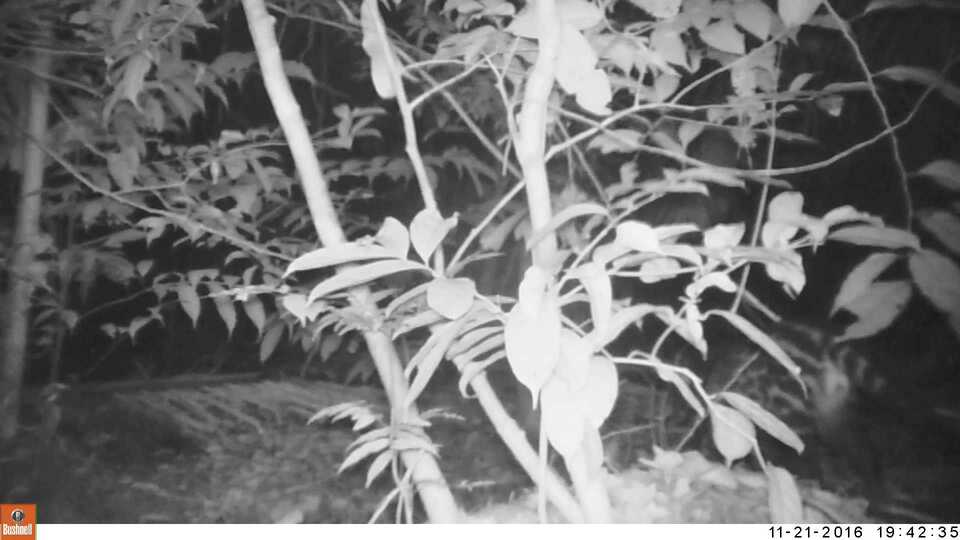
\includegraphics[width=65mm]{images/example_images/ZJ016488.jpg} & 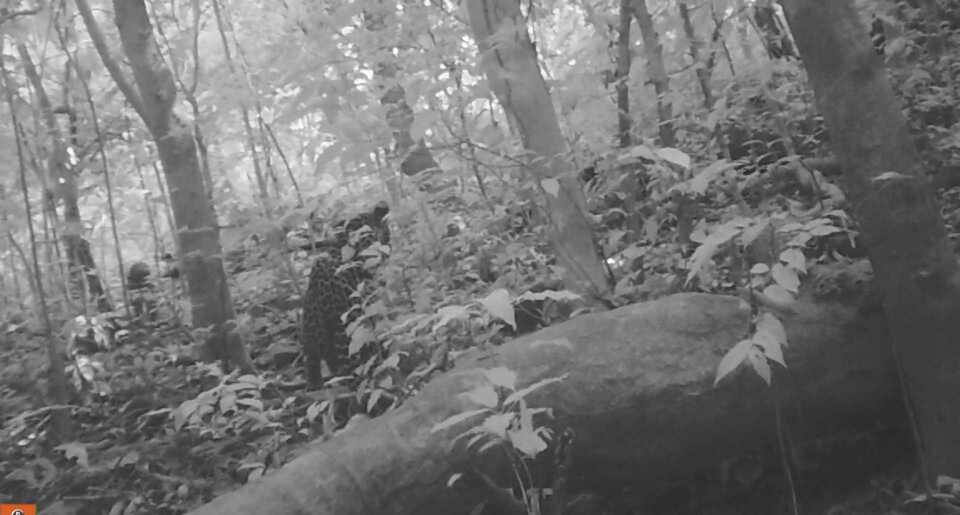
\includegraphics[width=65mm]{images/example_images/ZJ016498.jpg} \\
Beispielbild 1 & Beispielbild 2 \\[6pt]
 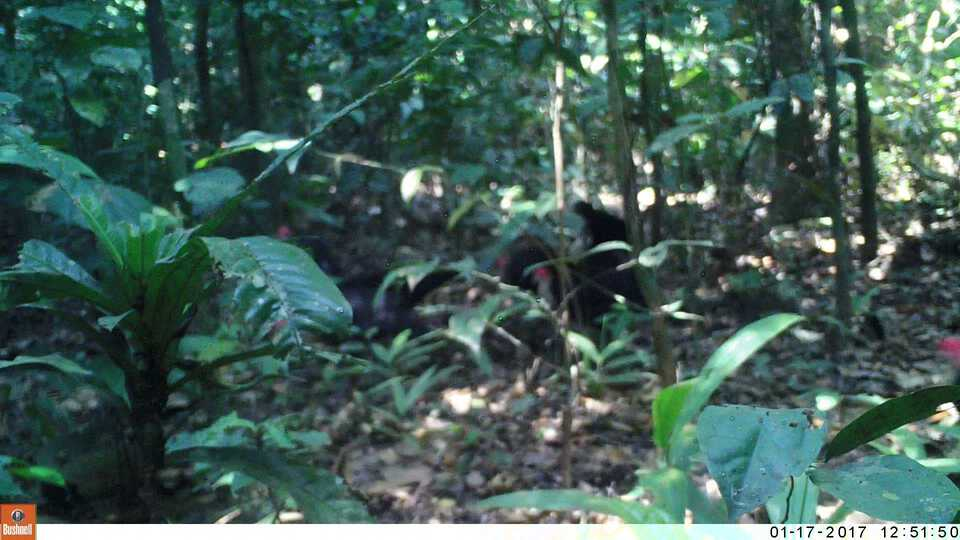
\includegraphics[width=65mm]{images/example_images/ZJ016503.jpg} & 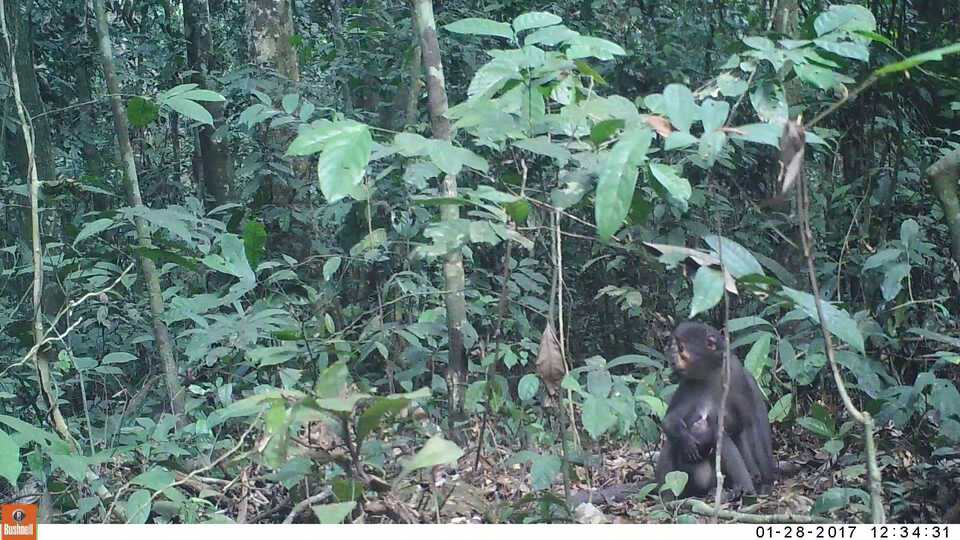
\includegraphics[width=65mm]{images/example_images/ZJ016535.jpg} \\
Beispielbild 3 & Beispielbild 4 \\[6pt]
 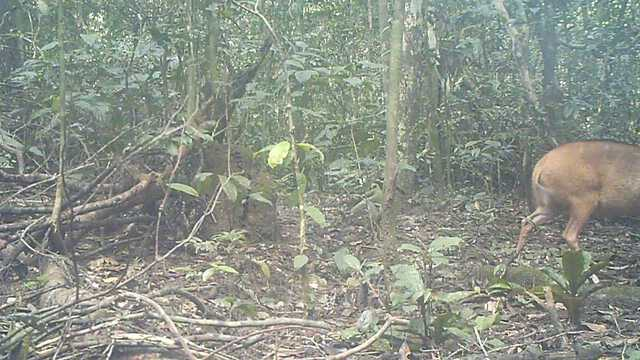
\includegraphics[width=65mm]{images/example_images/ZJ016561.jpg} & 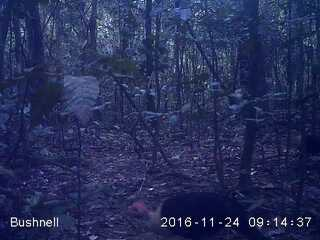
\includegraphics[width=65mm]{images/example_images/ZJ016556.jpg} \\
Beispielbild 5 & Beispielbild 6 \\[6pt]
\end{tabular}
\caption{\label{fig:random_pictures}Beispielbilder im Datensatz}
\end{figure}

Die ersten beiden Beispiele sind schwarz/weiss Bilder. Das Beispielbild 1 ist leicht überbelichtet und das Tier ist nur teilweise ersichtlich. Beim Beispielbild 2 ist zwar die Bildqualität gut, jedoch ist auch hier nur ein Teil des Tiers sichtbar. Im Beispielbild 3 sind nur die Blätter im Vordergrund scharf und das Tier ist unscharf. Beispielbild 4 ist ein relativ gutes und wahrscheinlich leicht zu klassifizierendes Bild, da das Tier voll sichtbar ist und die Bildqualität hoch ist.
Beim Beispielbild 5 läuft das Tier aus dem Bild, es ist nur zur Hälfte zu sehen. Im Beispielbild 6 ist die Beleuchtung anders als in den vorherigen Beispielbildern, was auf die Uhrzeit der Aufnahme zurückzuführen ist. Das Tier ist zwar erkennbar, jedoch ist die Bildqualität nicht besonders gut, ausserdem sieht man auf diesem Bild Metadaten als Text, was eine potenzielle Problemquelle für die Modelle sein könnte.

\subsection{Erste Analyse der Daten}

\begin{figure}[!h]
    \centering
    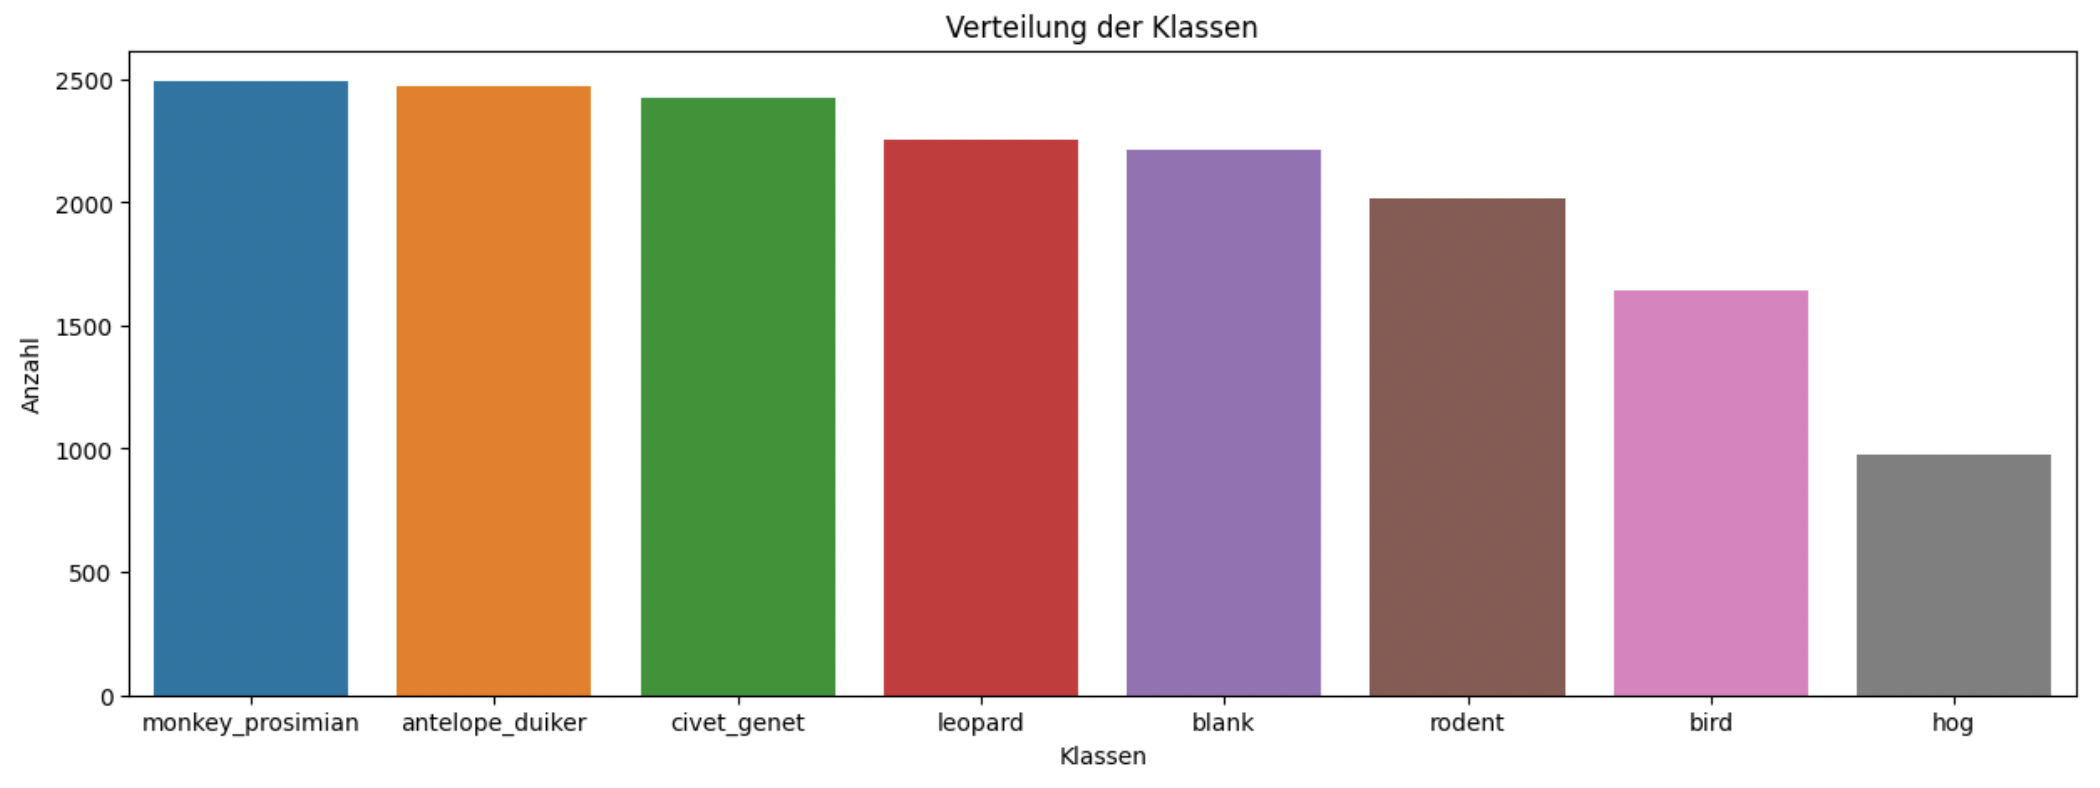
\includegraphics[width=12cm]{plots/Verteilung Klassen.png}
    \caption{\label{fig:nimber_of_images_per_class}Vorkommen der einzelnen Klassen.}
\end{figure}

Die Analyse der Verteilung der Klassen hat ergeben, dass die einige der Klassen ähnlich häufig vorkommen. Die Klassen 'monkey\_prosimian', 'antelope\_duiker' und 'civet\_gener' kommen alle sehr häufig im Datensatz vor. Die Klassen 'leopard', 'blank' und 'rodent' kommen bereits weniger oft vor, aber immer noch in einem Ausmass, wo wir keinen grossen Einfluss bei der Modellierung erwarten. Die Klasse 'bird' kommt schon weniger als die anderen Klassen vor und die Klasse 'hog' kommt dann deutlich am seltensten vor.

\begin{figure}[!h]
    \centering
    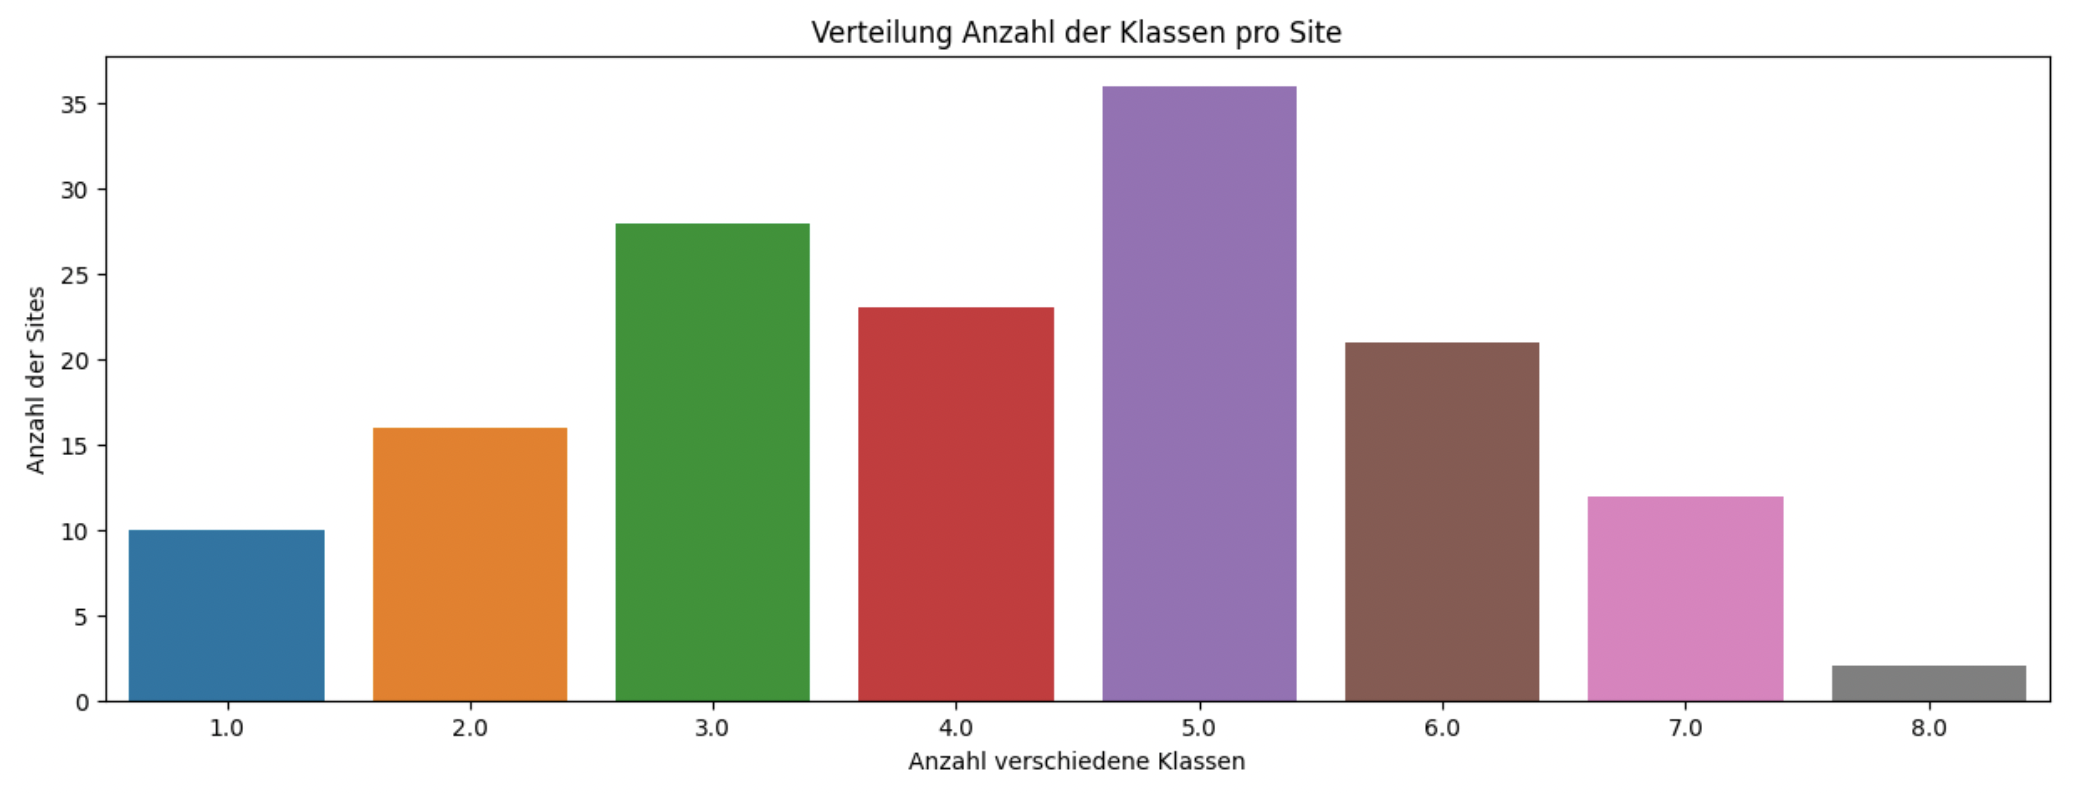
\includegraphics[width=10cm]{plots/Tierarten pro Location.png}
    \caption{\label{fig:number_of_animals_per_location}Anzahl Tierarten pro Location}
\end{figure}

\noindent
Die Untersuchung der Locations hat ergeben, dass bei den meisten zwischen drei und fünf Tierarten vorkommen. Der maximale Wert liegt bei acht Arten. Diese Erkenntnis ist wichtig, da eine gute Verteilung verhindert, dass das Modell eine Position der Kamera nicht als Feature einer Tierklasse erkennt. Dies gewinnt zusätzlich an Bedeutung, da bei der Challenge Locations nur entweder im Trainings- oder Testdatensatz vorkommen.\\\\

\newpage

\begin{figure}[!h]
    \centering
    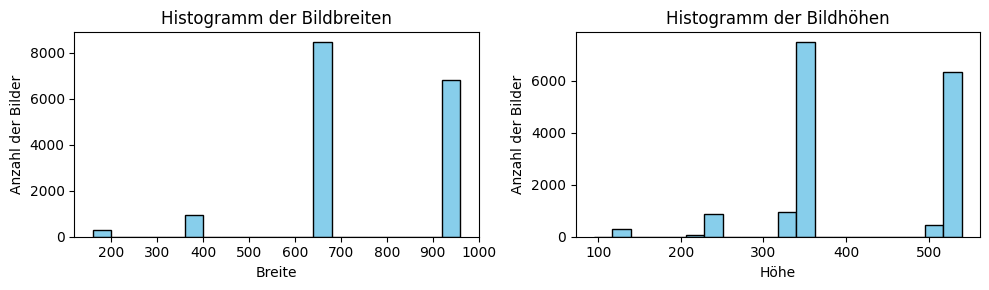
\includegraphics[width=10cm]{plots/Groesse der Bilder.png}
    \caption{\label{fig:size_distribution_of_pictures}Verteilung der Grössen der Bilder}
\end{figure}

\noindent
Die meisten Bilder sind 650 und 950 Pixel breit und 350 und 550 Pixel hoch. Es kristallisiert sich diesbezüglich keine universelle Gemeinsamkeit bei den Bildern hervor. Da wir in diesem Fall ohnehin ein Resizing der Bilder vornehmen müssen, werden wir vorwiegend die Grössen der Daten untersuchen, auf deren das jeweilige Modell vortrainiert wurde.

\begin{figure}[!h]
    \centering
    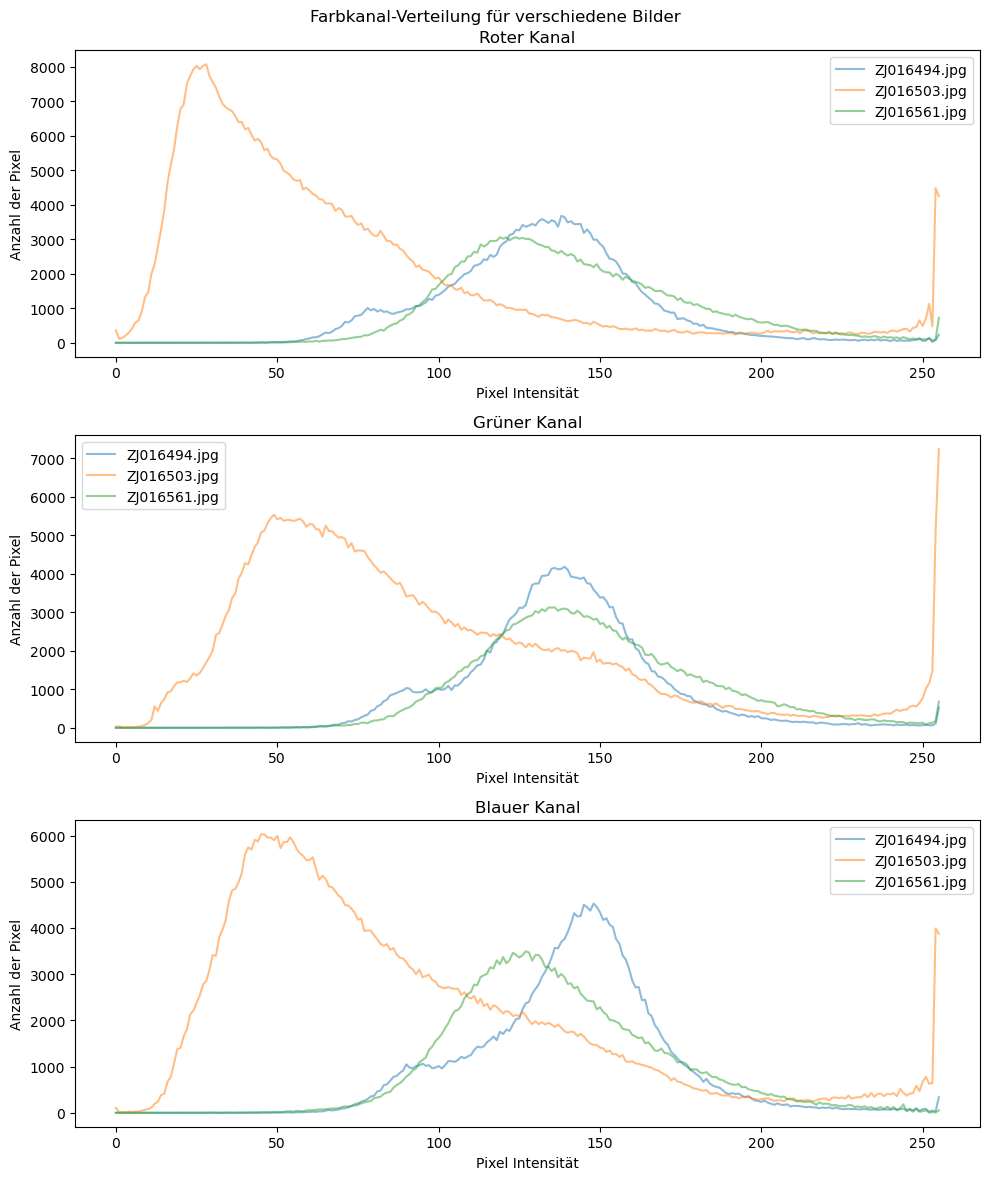
\includegraphics[width=10cm]{plots/Hist Farbe Vergleich.png}
    \caption{\label{fig:color_channels_of_3_pictures}Vergleich der Farbkanäle dreier zufällig ausgewählter Bilder}
\end{figure}

\noindent
Beim Vergleich der Farbkanäle drei zufälliger Bilder stellen wir fest, dass es einen starken Unterschied bei den Bildern gibt. Die Farbkanäle der Bilder prägen sich alle in unterschiedliche Richtungen aus. Dies könnte zum Problem werden, da die Möglichkeit besteht, dass sich die Modelle auf falsche Eigenschaften der Bilder fokussieren, falls dahingehend ein Zusammenhang mit den verschiedenen Tierklassen besteht. Andererseits ist es auch möglicherweise ein zusätzliches Attribut, woraus die Modelle Informationen extrahieren können. Wie sich die Modelle dementsprechend verhalten, wird sich bei der Modellierung zeigen. 

\newpage

\begin{figure}[!h]
    \centering
    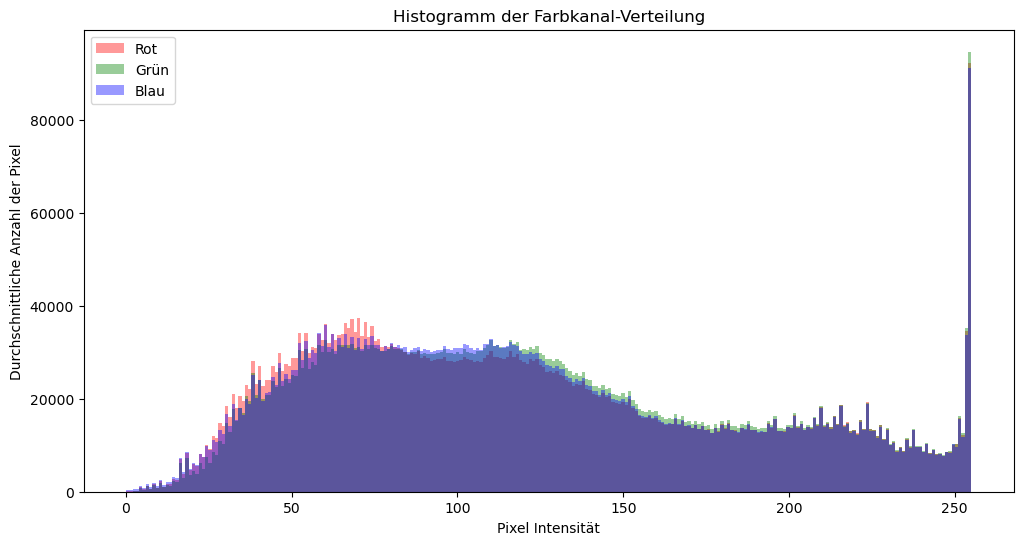
\includegraphics[width=10cm]{plots/Hist Farbe Mittelwert.png}
    \caption{\label{fig:average_color_channels}Histogramm der gemittelten Farbkanäle aller Bilder}
\end{figure}

\noindent
Über den Datensatz hinweg scheinen sich die Farbwerte jedoch relativ gleichmässig zu verteilen. Es zeigt sich also, dass keiner der drei Farbkanäle sich speziell auszuprägen scheint. Am rechten Rand des Histogramms wird ersichtlich, dass einige Bilder sehr helle Pixel ausweisen, was auf eine Überbelichtung dieser Bilder hindeutet.

\subsection{Probleme und Herausforderungen}

Folgende potenziellen Herausforderungen für die Challenge sind uns bei der Datenanalyse aufgefallen:\\

\noindent
\textbf{Bildqualität}\\
Eine Herausforderung besteht bei der Qualität und Konsistenz der Bilder. Die Bilder wurden von Wildtierkameras aufgenommen, die bei unterschiedlichen Licht- und Wetterbedingungen arbeiten. Einige Bilder waren daher unterbelichtet, überbelichtet, unscharf oder durch Wetterbedingungen wie Regen beeinträchtigt. In manchen Fällen war das Tier nur teilweise sichtbar oder sehr klein im Vergleich zum Hintergrund, was die Identifikation und Klassifizierung erschwert.\\

\noindent
\textbf{Unausgeglichene Klassen}\\
Ein weiteres Problem ist das Ungleichgewicht in den Klassen. Einige Tierarten ('monkey\_prosimian', 'antelope\_duiker') sind in den Bildern viel häufiger vertreten als andere (insbesondere 'hog'). Diese Unausgewogenheit kann dazu führen, dass die Modelle dazu neigen, die Mehrheitsklassen zu bevorzugen und die Minderheitsklassen zu übersehen, was zu einer ungenauen Klassifikation führt. Wir gehen davon aus, dass das Ungleichgewicht nicht stark genug ist, um das Training stark zu beeinflussen.\\
 
\noindent
\textbf{Position und Ausrichtung der Tiere}\\
Tiere werden in den Bildern in verschiedenen Positionen und Ausrichtungen dargestellt. Diese Variationen können die Fähigkeit des Modells zur korrekten Klassifizierung beeinträchtigen.\\

\newpage

\section{Methoden}

\subsection{Hardware \& Software}

\begin{itemize}
 \item Experiment Tracking: \textbf{Weights \& Biases}\\
 Dieses Tool dient dazu, um die Metriken, Resultate und Predictions zu loggen. Wir haben auch die Übersicht, welche Modelle mit welchen Hyperparameter zu welchem Resultat geführt haben.
 \item ML Framework: \textbf{Pytorch Lightning}\\
 Das Pytorch Lightning Framework bringt eine klassenbasierte Struktur in ein Deep Learning Projekt. Ausserdem bietet es eine einfache Integration in Weights \& Biases und eliminiert einen Grossteil des Boilerplate-Codes aus dem Projekt.
 \item Hardware: \textbf{Private GPU Hardware und CSCS}\\
 Primär wurden beim Trainieren private GPUs verwendet. Zusätzlich wurde teils das Swiss National Super Computing Center (CSCS) verwendet.
 \item Versionsverwaltung: \textbf{Gitlab}\\
 Die Versionskontrolle des Quellcodes erfolgt auf einem GitLab Repository auf der Instanz der FHNW. Mit dieser und insbesondere Funktionen zum Projektmanagement  ermöglicht es GitLab uns, effizient und synchron an der Software zu arbeiten.
 \item Projektmanagement: \textbf{Gitlab Boards}\\
 GitLab Boards direkt im Repository wurden verwendet, um Tickets und den Projektfortschritt zu verwalten. Es konnte auch der Fortschritt von Aufgaben verfolgt und bei abgeschlossenen Tickets Branches gemerged werden.
 \item Kommunikation im Team: \textbf{In Person}\\
 Primär fand der Austausch in Person an der FHNW statt. Koordiniert wurde per Messenger-App.
 \item Bericht: \textbf{Overleaf}\\
 Der Bericht wurde mit einer selbst gehosteten Instanz von Overleaf geschrieben. Overleaf ist eine Plattform für das Schreiben, Bearbeiten und Veröffentlichen von LaTeX-Dokumenten, die oft in akademischen und wissenschaftlichen Bereichen genutzt werden. 
 \item Virtual Environment: \textbf{Conda}\\
 Conda ist ein Virtual Enviroment Plattform von Anaconda. Es erleichtert die Arbeit mit Deep Learning Libraries und erlaubt es uns das Environment und die dazugehörigen Repositories in einem yml File bereitzustellen.
 \item Gitlab Struktur: \textbf{"Cookiecutter Data Science}\\
 Das Cookiecutter Data Science von DrivenData wurde als Template für die Ordnerstruktur verwendet. Dies stellt eine einheitliche Struktur in unserem Projekt sicher.

\end{itemize}

\newpage
\subsection{Optimizer}

Der Optimizer ist eine Schlüsselkomponente, die die Lernmethode für ein Deep Learning Modell bestimmt. Seine Aufgabe besteht darin, die Gewichte und Bias-Werte des Netzwerks anzupassen, um den Verlust (Loss) zu minimieren und somit die Genauigkeit der Vorhersagen zu maximieren.\\\\
Die Arbeit eines Optimierers beruht auf dem Konzept des Gradientenabstiegs. In einem hochdimensionalen Raum sucht der Optimierer nach der Richtung, in der die Funktion (der Verlust) am schnellsten abnimmt und nimmt dann Schritte in diese Richtung, um den minimalen Verlust zu erreichen. Dieser Prozess wird wiederholt, bis eine bestimmte Bedingung erfüllt ist – beispielsweise eine festgelegte Anzahl von Iterationen oder bis der Verlust einen bestimmten Wert erreicht.\\\\
Ein Optimierer muss effizient sein, um den Prozess des Trainings zu beschleunigen, aber auch präzise, um eine angemessene Leistung des Modells sicherzustellen.\\\\
Schliesslich ermöglicht der Optimierer in Deep Learning auch die Implementierung von Regularisierungs-Techniken, wie L1 und L2 Regularisierung oder Dropout, die dazu beitragen können, das Überanpassen (Overfitting) zu vermeiden, und hilft, die Robustheit des Modells zu verbessern.

\subsubsection{Stochastic Gradient Descent (SGD)}

Stochastic Gradient Descent (SGD) ist eine Optimierungsmethode, die in vielen Machine-Learning- und Deep-Learning-Algorithmen verwendet wird, um die Parameter eines Modells zu aktualisieren und zu optimieren, um die Genauigkeit der Vorhersagen zu maximieren.\\\\
Der SGD-Algorithmus arbeitet auf die gleiche Weise wie der herkömmliche Gradientenabstieg, verwendet jedoch nur einen einzigen, zufällig ausgewählten Datenpunkt (oder eine kleine Gruppe von Datenpunkten, bekannt als Minibatch), um den Gradienten bei jeder Iteration zu berechnen, anstatt das gesamte Datenset zu verwenden. Diese Methode macht den Algorithmus wesentlich schneller und ermöglicht es, auch bei sehr grossen Datensätzen effizient zu arbeiten.

\begin{figure}[!h]
    \centering
    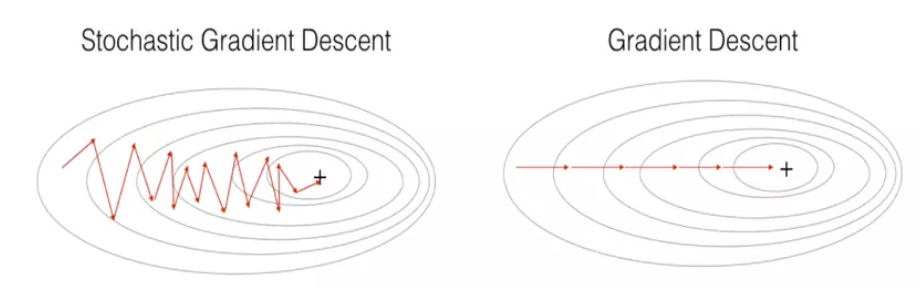
\includegraphics[width=0.8\textwidth]{images/sgd.png}
    \caption{\label{fig:resnet_50_architecture}Stochastic Gradient Descent Illustration (Quelle: \href{https://stackoverflow.com/questions/69251109/fluctuations-of-gradient-descent}{Stackoverflow})}
\end{figure}


Das Verfahren des Stochastic Gradient Descent beginnt mit der zufälligen Initialisierung der Modellparameter. Anschliessend wird eine zufällige Dateninstanz oder ein Minibatch aus dem Trainingssatz ausgewählt. Auf der Grundlage dieser einzelnen Dateninstanz oder des Minibatches wird der Gradient des Verlusts in Bezug auf die Parameter des Modells berechnet. Die Modellparameter werden dann in Richtung des negativen Gradienten aktualisiert, um den Verlust zu minimieren. Dies geschieht unter Verwendung eines als «Lernrate» bezeichneten Hyperparameters, der bestimmt, wie weit wir in Richtung des negativen Gradienten gehen. Diese Schritte werden für eine bestimmte Anzahl von Iterationen wiederholt, oder bis der Verlust unter einen bestimmten Schwellenwert sinkt oder aufhört, sich zu verbessern.\\\\
Während SGD effizient ist, kann es auch instabil sein, da die Verwendung von nur einer einzelnen Dateninstanz oder eines Minibatches dazu führen kann, dass der Gradientenabstieg in verschiedene Richtungen "springt". Um dieses Problem zu mildern, werden oft Variationen von SGD verwendet, die zusätzliche Techniken wie Momentum oder adaptives Lernen einsetzen.

\subsubsection{Adam}

Adam \cite{kingma_adam_2017}, was für "Adaptive Moment Estimation" steht, ist ein Optimierungsalgorithmus, der in vielen Deep-Learning-Anwendungen verwendet wird. Er wurde entwickelt, um die Geschwindigkeit und Leistung des Stochastic Gradient Descent (SGD) zu verbessern.\\\\
Im Gegensatz zu SGD, das einfach den rohen Gradienten verwendet, um die Parameteraktualisierungen durchzuführen, verwendet Adam sowohl den ersten Moment (das ist im Grunde der Durchschnitt) als auch den zweiten Moment (die ungefähre Varianz) der Gradienten, um die Parameteraktualisierungen zu berechnen. Diese zusätzlichen Informationen helfen Adam dabei, die Lernrate für jeden Parameter individuell anzupassen, was zu effizienteren und stabilen Updates führt.\\\\
Adam beginnt seine Arbeit mit der Initialisierung der Modellparameter und setzt sowohl den ersten als auch den zweiten Moment auf null. In jedem Schritt des Trainings wird eine Dateninstanz oder ein Minibatch aus dem Trainingssatz zufällig ausgewählt. Mit diesen Daten wird der Gradient des Verlusts in Bezug auf die Parameter berechnet.\\\\
Adam aktualisiert dann die Schätzungen des ersten und des zweiten Moments, indem er einen laufenden Durchschnitt der Gradienten und ihrer quadrierten Werte bildet. Diese Schätzungen werden korrigiert, um den Bias zu reduzieren, der sich durch den Anfang bei null ergibt.\\\\
Die Modellparameter werden dann unter Berücksichtigung dieser korrigierten Momenten-schätzungen aktualisiert. Dies bedeutet, dass Parameter, die grössere Gradientenwerte aufweisen (was darauf hindeutet, dass sie einen grösseren Einfluss auf den Verlust haben), stärkere Anpassungen erfahren als solche mit kleineren Gradienten.\\\\
Dieser Prozess wird wiederholt, bis der Verlust unter einen bestimmten Schwellenwert sinkt, bis eine festgelegte Anzahl von Iterationen erreicht ist oder bis der Verlust aufhört, sich zu verbessern.\\\\
Eine der Stärken von Adam besteht darin, dass er sowohl die Vorteile des Momentum (durch den ersten Moment) als auch die des adaptiven Lernens (durch den zweiten Moment) kombiniert, was ihn zu einem sehr effizienten und robusten Optimierer für viele Deep-Learning-Aufgaben macht.

\subsubsection{AdamW}
AdamW \cite{loshchilov_decoupled_2019} ist eine Variation des Adam-Optimierers, die für Deep Learning-Projekte verwendet wird. Wie Adam kombiniert auch AdamW die Konzepte des ersten und zweiten Moments, also den Durchschnitt und die Varianz der Gradienten, um effektive Updates der Modellparameter zu ermöglichen. Der entscheidende Unterschied besteht darin, wie AdamW die Gewichtsregularisierung behandelt.\\\\
Die Gewichtsregularisierung ist eine Technik, die dazu dient, Overfitting zu vermeiden, indem sie die Komplexität des Modells beschränkt. Dies wird oft erreicht, indem ein zusätzlicher Term zur Verlustfunktion hinzugefügt wird, der die Grösse der Modellparameter bestraft. In der ursprünglichen Adam-Implementierung wurde diese Regularisierung direkt in den Gradientenschritt eingebettet.\\\\
AdamW ändert diesen Ansatz, indem es die Regularisierung und die Parameteraktualisierung trennt. Es führt die Gewichtsaktualisierung in zwei Schritten durch: zuerst wird ein Schritt mit unregulierten Gradienten unternommen (wie in der ursprünglichen Adam-Formulierung), dann wird ein Schritt unternommen, der die Gewichtsregularisierung berücksichtigt.\\\\
Die Arbeit mit AdamW beginnt mit der Initialisierung der Modellparameter und dem Setzen der ersten und zweiten Momente auf null. In jedem Trainingsschritt wird eine Dateninstanz oder ein Minibatch aus dem Trainingssatz ausgewählt. Mit diesen Daten wird der Gradient des Verlustes in Bezug auf die Parameter berechnet.\\\\
AdamW aktualisiert dann die Schätzungen des ersten und des zweiten Moments, indem er einen laufenden Durchschnitt der Gradienten und ihrer quadrierten Werte bildet. Diese Schätzungen werden korrigiert, um den Bias zu reduzieren, der sich durch den Anfang bei null ergibt.\\\\
Anschliessend werden die Modellparameter zunächst unter Berücksichtigung dieser korrigierten Momenten-schätzungen aktualisiert. Danach wird ein Schritt unternommen, der die Gewichtsregularisierung berücksichtigt, wobei die Parameter in Abhängigkeit von ihrer Grösse weiter angepasst werden.\\\\
Dieser Prozess wird wiederholt, bis der Verlust unter einen bestimmten Schwellenwert sinkt, bis eine festgelegte Anzahl von Iterationen erreicht ist, oder bis der Verlust aufhört, sich zu verbessern.\\\\
Die Trennung der Gewichtsaktualisierung und der Regularisierung, wie sie in AdamW implementiert ist, hat sich in der Praxis als vorteilhaft erwiesen und kann zu besseren Trainingsergebnissen führen als die ursprüngliche Adam-Formulierung, insbesondere bei tiefen und komplexen Modellen.

\subsubsection{Vergleich}

Im Laufe der Challenge haben wir parallel zu unserem Lern-Prozess im Modul Deep Learning verschiedene Optimierungsalgorithmen verwendet und verglichen, um die bestmögliche Performance und Genauigkeit unseres Deep-Learning-Modells zu erzielen. Unser Weg führte uns von Stochastic Gradient Descent (SGD) über Adam hin zu AdamW.\\\\
Wir begannen unsere Arbeit mit SGD, einem klassischen Optimierungsverfahren, das auf dem Prinzip des Gradientenabstiegs basiert. Obwohl wir anfangs gute Fortschritte mit SGD erzielt haben, fanden wir, dass der Algorithmus manchmal instabil sein kann und dazu neigt, in verschiedene Richtungen zu "springen", was zu langsamer Konvergenz und weniger präzisen Ergebnissen führen kann.\\\\
Um diese Herausforderungen zu bewältigen, haben wir uns entschieden, zu Adam zu wechseln. Die zusätzlichen Informationen des ersten und zweiten Moment der Gradienten ermöglichen es Adam, die Lernrate für jeden Parameter individuell anzupassen, was zu effizienteren und stabileren Updates führt. Nach dem Wechsel zu Adam bemerkten wir, dass unsere Modelle deutlich schneller konvergieren.\\\\
Trotz dieser Verbesserungen mit Adam haben wir festgestellt, dass wir einen Teil der Präzision, die wir mit SGD hatten, verloren haben. Um dies zu beheben, haben wir uns entschieden, teilweise auf AdamW umzusteigen, eine Variation von Adam, die die Behandlung der Gewichtsregularisierung ändert. Diese Modifikation hat es uns ermöglicht, einen Teil der Präzision, die wir ursprünglich mit SGD hatten, zurückzugewinnen, während wir die verbesserte Performance von Adam beibehalten.

\newpage

\subsection{Metriken und Verlustfunktionen}
Metriken und Verlustfunktionen fassen die Leistung eines Modells in eine oder mehrere Zahlen zusammen, um diese objektiv untereinander vergleichen zu können. Da die DrivenData Challenge auf der Log Loss Verlustfunktion basiert, wird diese sicher ein Fokus bei der Entwicklung sein. Zusätzlich evaluieren wir noch eine weitere Metrik, den F1 Score, welche für uns Menschen leichter verständlich ist als eine logarithmische Verlustfunktion.

\subsubsection{Log Loss}

Die Logarithmische Verlustfunktion (Log Loss) ist eine wichtige Methode zur Evaluierung von Modellen, die Wahrscheinlichkeitsvorhersagen für mehrere Klassen liefern, wie Multinomial logistische Regression und viele Arten von neuronalen Netzen. Es handelt sich dabei um eine negative log-likelihood Funktion.\\
Die Formel für die Verlustfunktion sieht dabei folgendermassen aus:

\[
\text{loss} = -\frac{1}{N} \sum_{i=1}^{N} \sum_{j=1}^{M} y_{ij} \log(p_{ij})
\]

\noindent
\textbf{N} steht für die Anzahl der Beobachtungen oder Datenpunkte.\\
\textbf{M} steht für die Anzahl der möglichen Klassen.\\
$\mathbf{y_{ij}}$ ist eine binäre Indikatorvariable, die 1 ist, wenn die Beobachtung i zu Klasse j gehört, und sonst 0.\\
$\mathbf{p_{ij}}$ ist die vorhergesagte Wahrscheinlichkeit dafür, dass die Beobachtung i zu Klasse j gehört.\\\\

\noindent
Die Formel summiert über alle Beobachtungen und alle Klassen. Für jede Beobachtung-Klasse-Paarung nimmt sie die tatsächliche Zugehörigkeit ($y_{ij}$) und multipliziert sie mit dem Logarithmus der vorhergesagten Wahrscheinlichkeit ($p_{ij}$). Wenn die tatsächliche Zugehörigkeit 1 ist, wird der Logarithmus der vorhergesagten Wahrscheinlichkeit in die Summe einbezogen. Wenn die tatsächliche Zugehörigkeit 0 ist, wird nichts in die Summe einbezogen, da 0 multipliziert mit etwas immer 0 ist.\\\\
Dieser Gesamtwert wird dann durch -1/N multipliziert, um den Durchschnittsverlust pro Beobachtung zu berechnen. Das Minuszeichen ist da, weil die Logarithmen von Wahrscheinlichkeiten zwischen 0 und 1 immer negative Zahlen sind, und wir wollen einen positiven Verlustwert.\\\\
Der Log Loss hat eine interessante Eigenschaft: Er bestraft nicht nur falsche Vorhersagen, sondern auch das Ausmass, in dem sie falsch sind. Zum Beispiel ist eine Vorhersage, die falsch ist, aber nahe an der Wahrheit liegt (z. B. Vorhersage=0.49, Wahrheit=0.5) weniger schlimm als eine, die weit entfernt ist (z. B. Vorhersage=0.1, Wahrheit=0.9). Dies macht den Log Loss zu einer guten Wahl, wenn man sich nicht nur dafür interessiert, ob Vorhersagen richtig oder falsch sind, sondern auch, wie zuversichtlich sie sind.

\newpage

\subsubsection{F1 Score}
Der F1-Score ist ein Mass für die Leistung eines Modells im Bereich der binären Klassifikation, aber es kann auch auf multiklassen Probleme angewandt werden. Er wird aus Precision (Genauigkeit) und Recall (Sensitivität) berechnet und versucht, ein Gleichgewicht zwischen beiden zu finden. Die Berechnung des F1-Scores ist 

\begin{equation}
F1 = 2 \cdot \frac{{\text{{Precision}} \cdot \text{{Recall}}}}{{\text{{Precision}} + \text{{Recall}}}}
\end{equation}
 
Bei der Erweiterung auf multiklassen Probleme haben wir drei gängige Varianten: Micro-F1, Macro-F1 und Weighted-F1.\\\\
\textbf{Micro-F1-Score}: Bei der Micro-Auswertung werden die Leistungen über alle Klassen hinweg aggregiert. Es wird eine Gesamtzahl an True Positives, False Positives und False Negatives berechnet und diese werden zur Berechnung von Precision, Recall und folglich des F1-Scores verwendet. Dies ist besonders nützlich, wenn der Datensatz eine ungleiche Verteilung der Klassen aufweist, da er die Leistung über alle Klassen hinweg misst.\\
\textbf{Macro-F1-Score}: Der Macro-F1-Score berechnet Precision, Recall und F1-Score für jede Klasse unabhängig voneinander und nimmt dann den Durchschnitt. Dies bedeutet, dass jede Klasse unabhängig von ihrer Grösse gleich gewichtet wird. Diese Methode kann zu einem schlechteren Ergebnis führen, wenn es im Datensatz eine Klasse mit vielen Beobachtungen gibt und eine andere Klasse mit nur wenigen Beobachtungen.\\
\textbf{Weighted-F1-Score}: Der Weighted-F1-Score ist ähnlich wie der Macro-F1-Score, jedoch wird jeder F1-Score entsprechend der Anzahl der Beobachtungen in jeder Klasse gewichtet, bevor der Durchschnitt berechnet wird. Dies bedeutet, dass die Klassen, die mehr Beobachtungen enthalten, stärker gewichtet werden. Diese Methode ist nützlich, wenn die Daten unausgeglichen sind, da sie der Klasse mit mehr Beobachtungen mehr Gewicht verleiht.

\newpage
\subsection{Verwendete Deep Learning Modelle}

Zu Beginn des Semesters hatten wir noch keine Erfahrung zur Arbeit mit Bildklassifizierungsmodellen. Als Startpunkt haben wir uns auf die vortrainierten Modelle von PyTorch, welche in die Torchvision Library eingebaut sind fokussiert, welche ein gutes Resultat in ImageNet, einem weitverbreiteten Benchmark für solche Modelle, erreichten (\href{https://pytorch.org/vision/stable/models.html#table-of-all-available-classification-weights}{PyTorch - Verfügbare Pretrained Weights}).

\subsubsection{ResNet-50}

\begin{figure}[!h]
    \centering
    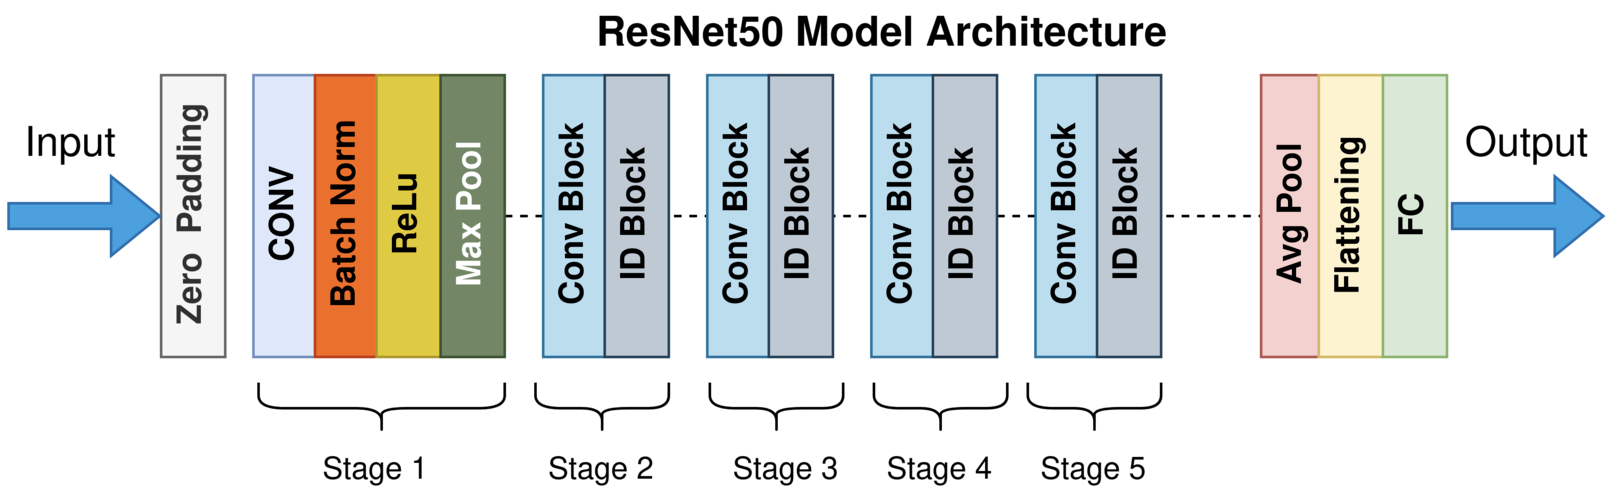
\includegraphics[width=0.8\textwidth]{images/model_architecture/resnet.png}
    \caption{\label{fig:resnet_50_architecture}Architektur des ResNet-50 Modells (Quelle: \href{https://commons.wikimedia.org/wiki/File:ResNet50.png}{Wikimedia})}
\end{figure}

ResNet-50 \cite{he_deep_2015} ist ein tiefes neuronales Netzwerk, das auf der ResNet-Architektur (Residual Network) basiert und 50 Schichten tief ist. Die Schlüsselinnovation von ResNet ist die Idee von "Residual Learning" oder "Shortcut Connections". Diese "Verknüpfungen" erlauben es dem Modell, die Ausgabe einer Schicht nicht nur als Eingabe für die nächste Schicht zu verwenden, sondern sie auch direkt weiter unten in der Netzwerkarchitektur zu nutzen. Diese Art von Verknüpfung hilft, das Problem des "verschwindenden Gradienten" zu bekämpfen, das häufig in sehr tiefen neuronalen Netzwerken auftritt.\\\\
Jede Residual Unit in ResNet besteht aus mehreren Schichten, normalerweise einem Convolution Layer, gefolgt von einer Batch Normalization Layer und einer ReLU (Rectified Linear Unit) Activation Layer. Bei ResNet-50 werden manchmal "bottleneck" Blöcke mit drei Schichten verwendet, um die Anzahl der Parameter zu reduzieren und die Rechenleistung zu verbessern.\\\\
Das Modell wird typischerweise für Bildklassifikationsaufgaben verwendet und kann mit einer grossen Menge an Daten trainiert werden, um Muster und Merkmale in den Bildern zu erkennen. Es wird oft als Backbone-Netzwerk für viele Computer-Vision-Aufgaben verwendet, da es sehr effizient ist und hervorragende Ergebnisse liefert. \\\\
Das ResNet-50 wurde bei dieser Competition als Benchmark-Modell verwendet. Daher haben wir uns anfangs entschieden den Benchmark zu Rekreieren und dann den zu versuchen, das bestmögliche aus dem Modell herauszuholen, um zu sehen, was wir am Benchmark noch verbessern können.


\newpage

\subsubsection{EfficientNetv2}

EfficientNetv2 \cite{tan_efficientnetv2_2021} ist eine Familie von skalierbaren Konvolutions-Neural-Netzwerken (CNNs), die für eine Reihe von Computer Vision-Aufgaben entwickelt wurde. Sie baut auf der ursprünglichen EfficientNet-Architektur auf, bietet jedoch Verbesserungen in Bezug auf Effizienz und Genauigkeit. EfficientNetv2 hat verschiedene Modelle in seiner Familie, die in Grösse und Kapazität variieren, um unterschiedliche Anforderungen in Bezug auf Rechenressourcen und Genauigkeit zu erfüllen.\\\\
Die Schlüsselinnovationen von EfficientNetv2 beinhalten die Verwendung eines effizienten Trainingsverfahrens, das als "progressive Learning" bezeichnet wird, und eine Reihe von Optimierungen, um die Effizienz der Netzwerkarchitektur zu verbessern. Progressives Learning beginnt mit einem kleinen Modell, das auf niedriger Auflösung trainiert wird, und vergrössert dann schrittweise das Modell und die Auflösung. Dieser Ansatz hilft, die Trainingseffizienz zu verbessern.\\\\
EfficientNetv2 verwendet ausserdem eine optimierte Mixtur von Convolutions (Faltungsschichten) einschliesslich Depthwise Convolutions und MBConv (Mobile Inverted Bottleneck Convolutions), um die Modellgrösse und die Anzahl der Rechenoperationen zu reduzieren, ohne die Leistung zu beeinträchtigen. Diese Anpassungen helfen, die Genauigkeit des Modells zu verbessern, während sie weniger Ressourcen verbrauchen, was sie ideal für Anwendungen auf Geräten mit begrenzten Ressourcen macht, wie z. B. Mobiltelefone. 


\subsubsection{DenseNet-161}

\begin{figure}[!h]
    \centering
    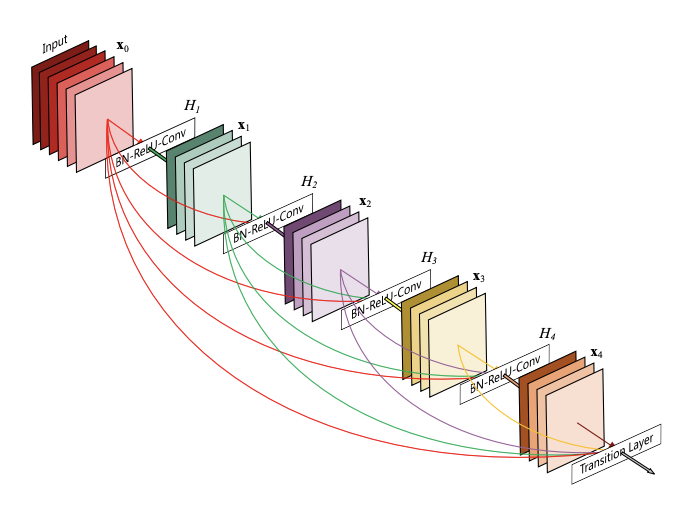
\includegraphics[width=0.5\textwidth]{images/model_architecture/densenet.png}
    \caption{\label{fig:resnet_50_architecture}Architektur des DenseNet-161 Modells (Quelle: \href{https://paperswithcode.com/lib/torchvision/densenet}{PapersWithCode})}
\end{figure}



DenseNet-161 \cite{huang_densely_2018} ist ein Deep Learning-Modell, das auf der Dense Convolutional Network (DenseNet) Architektur basiert und 161 Schichten tief ist. DenseNet ist für seine Dichte an Verbindungen zwischen den Schichten bekannt – im Gegensatz zu traditionellen Netzwerken, bei denen jede Schicht nur mit der nächsten verbunden ist, ist jede Schicht in DenseNet mit jeder nachfolgenden Schicht verbunden.\\\\
Der Schlüsselmechanismus in DenseNet ist die "Dense Connection". In einem dicht verbundenen Block erhält jede Schicht die Feature-Maps aller vorherigen Schichten als Eingabe und gibt ihre eigenen Feature-Maps an alle folgenden Schichten weiter. Diese Methode ermöglicht es dem Netzwerk, tiefe überwachte Signale zu haben und den Informationsfluss im Netzwerk zu verbessern, was zu besseren Ergebnissen führt und das Problem des "verschwindenden Gradienten" reduziert.\\\\
DenseNet-161 hat eine hohe Modellkapazität und ist daher gut geeignet für Aufgaben mit grosser Datenvielfalt und Komplexität, wie feingranulare Bildklassifikation oder Segmentierung. Es ist jedoch auch ressourcenintensiver als einige andere Modelle, da die dichten Verbindungen eine grössere Anzahl von Parametern und eine höhere Rechenlast erfordern.

\newpage

\subsubsection{VGG-19}
\begin{figure}[!h]
    \centering
    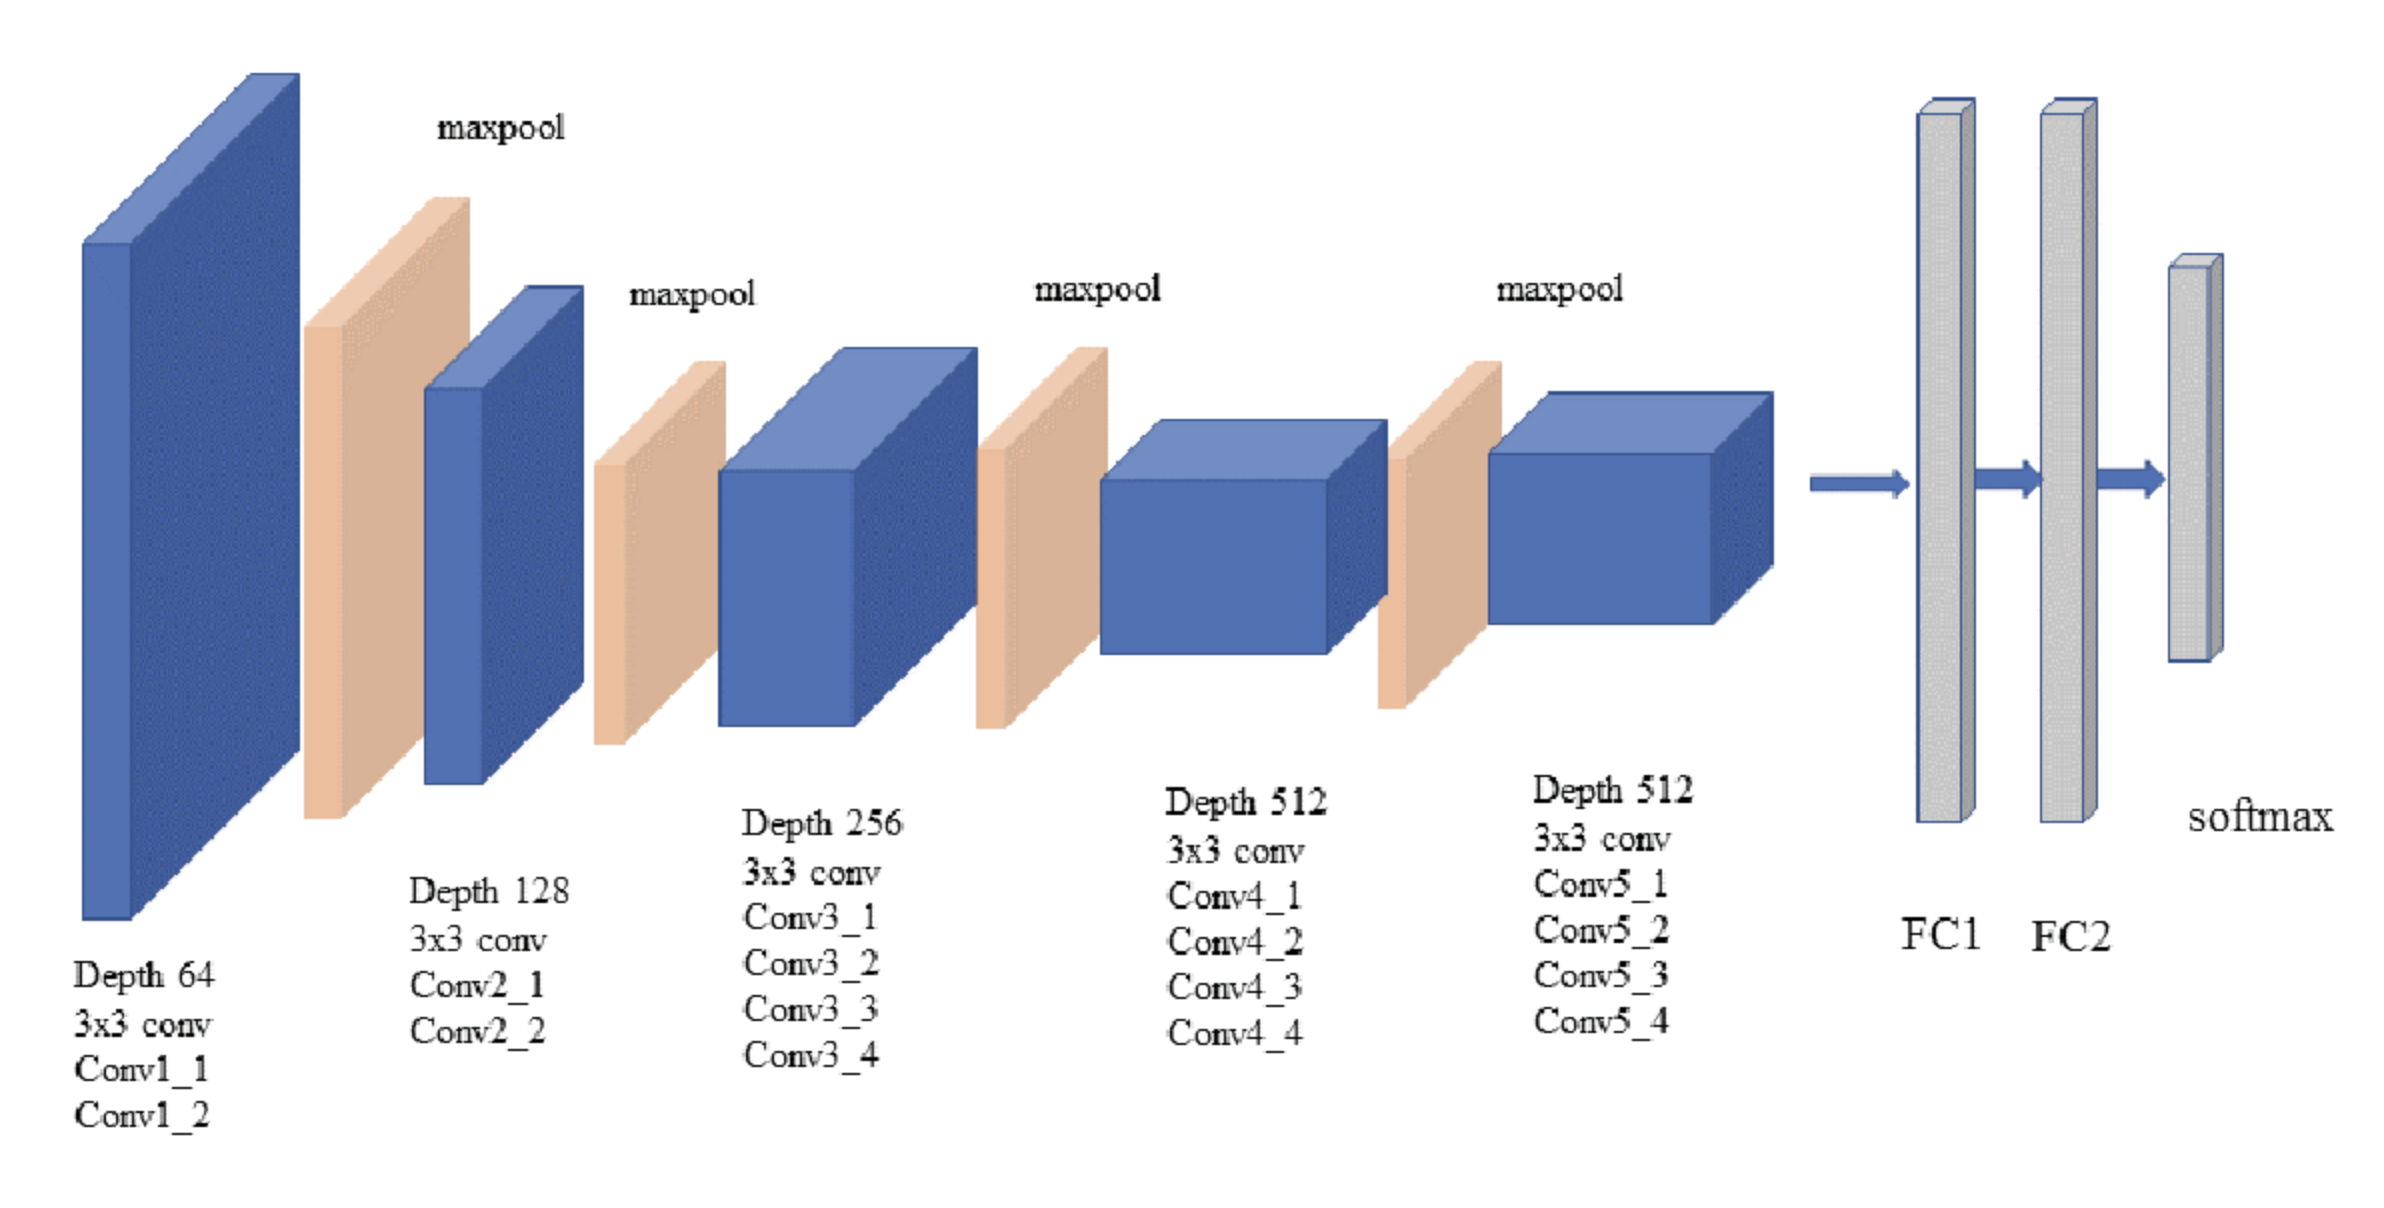
\includegraphics[width=0.5\textwidth]{images/model_architecture/vgg19.png}
    \caption{\label{fig:resnet_50_architecture}Architektur des VGG-19 Modells (Quelle: \href{https://towardsdatascience.com/extract-features-visualize-filters-and-feature-maps-in-vgg16-and-vgg19-cnn-models-d2da6333edd0}{TowardsDataScience})}
\end{figure}

VGG-19 \cite{simonyan_very_2015} ist ein Deep Learning-Modell, das auf der Visual Geometry Group (VGG) Netzwerkarchitektur basiert und 19 Schichten tief ist. Diese Architektur wurde von der Visual Geometry Group an der University of Oxford entwickelt, daher der Name. VGG-19 besteht aus 16 konvolutionellen Schichten, gefolgt von 3 vollständig vernetzten Schichten. Alle versteckten Schichten verwenden die ReLU (Rectified linear Unit) Aktivierungsfunktion.\\\\
Die Hauptinnovation von VGG-19 besteht darin, eine grosse Anzahl von Schichten mit kleinen, 3x3 Convolution Kernels zu verwenden. Diese kleinen Kernels ermöglichen es dem Modell, eine Vielzahl von Merkmalen in den Eingabebildern zu erfassen, während sie im Vergleich zu grösseren Kernels weniger Parameter erfordern.\\\\
VGG-19 wurde ursprünglich für Bildklassifikations- und Lokalisierungsaufgaben trainiert, ist aber auch in einer Vielzahl anderer Anwendungen nützlich, einschliesslich Transfer Learning und Feature Extraction. Es ist bekannt für seine einfache und leicht zu verstehende Architektur sowie seine hervorragende Leistung, allerdings hat es im Vergleich zu neueren Modellen eine relativ hohe Anzahl von Parametern und benötigt daher mehr Speicherplatz und Rechenzeit.

\subsubsection{InceptionV3}

InceptionV3 \cite{szegedy_rethinking_2015} ist ein Deep Learning-Modell, das auf der Inception-Netzwerkarchitektur basiert und speziell für Bildklassifikationsaufgaben entwickelt wurde. Es handelt sich um die dritte Iteration der Inception-Modelle, die von Forschern bei Google entwickelt wurden.\\\\
Der Schlüssel zur Inception-Architektur ist das sogenannte "Inception-Modul". In einem Inception-Modul werden verschiedene Arten von Convolution-Layern (z. B. 1x1, 3x3, 5x5) und Pooling-Layern parallel ausgeführt und ihre Ergebnisse anschliessend zusammengefügt. Dies ermöglicht es dem Netzwerk, Merkmale auf verschiedenen Skalen zu erfassen und die Rechenlast zu optimieren.\\\\
InceptionV3 führt auch mehrere Verbesserungen seinen Vorgängern gegenüber ein. Es verwendet Faktorisierung, um die Anzahl der Parameter in den Netzwerkschichten zu reduzieren, und enthält zusätzliche Seitenausgänge, um das Netzwerk während des Trainings zu regulieren und zu verhindern, dass Gradienten verschwinden oder explodieren. Dies macht InceptionV3 effizienter und genauer als seine Vorgänger. Es ist bekannt für seine hohe Genauigkeit bei Bildklassifikationsaufgaben, ohne eine extrem grosse Anzahl von Parametern zu benötigen.

\newpage
\subsubsection{Vision Transformer (ViT)}

\begin{figure}[!h]
    \centering
    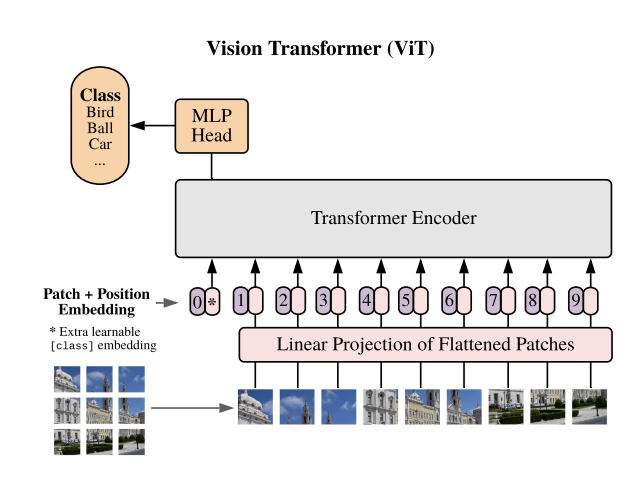
\includegraphics[width=0.4\textwidth]{images/model_architecture/vit.png}
    \caption{\label{fig:resnet_50_architecture}Vision Transformer Architektur (Quelle: \href{https://paperswithcode.com/method/vision-transformer}{PapersWithCode})}
\end{figure}

Der Vision Transformer (ViT) \cite{dosovitskiy_image_2021} ist ein Deep Learning-Modell, das auf der Transformer-Architektur basiert und speziell für Bildklassifikationsaufgaben entwickelt wurde. Es wurde von Forschern bei Google vorgeschlagen und stellt eine grundlegende Abkehr von bisherigen, auf Convolution basierenden Netzwerkarchitekturen dar.\\\\
Die Schlüsselinnovation von ViT ist die Anwendung der Transformer-Architektur, die ursprünglich für natürliche Sprachverarbeitungsaufgaben entwickelt wurde, auf Computer Vision-Aufgaben. ViT teilt das Eingabebild in eine Anzahl fester Grösse von Patches, die als Sequenz behandelt werden - ähnlich wie Wörter in einem Text. Diese Patches werden dann durch einen Transformer geleitet, der die Beziehungen zwischen ihnen lernt.\\\\
Das spezifische Modell "vit-large-patch16-224-in21k" ist eine Variante des Vision Transformers, die von Google bereitgestellt wird. Hier steht "large" für die Grösse des Modells, "patch16" bedeutet, dass das Eingabebild in Patches der Grösse 16x16 aufgeteilt wird, "224" bezieht sich auf die Grösse der Eingabebilder (224x224 Pixel) und "in21k" deutet darauf hin, dass das Modell anfangs auf einem Datensatz mit 21 Tausend verschiedenen Klassen trainiert wurde. Trotz der hohen Rechenanforderungen dieser Modelle haben sie gezeigt, dass sie ähnliche oder bessere Ergebnisse als herkömmliche CNNs liefern können.

\newpage
\begin{figure}[!h]
    \centering
    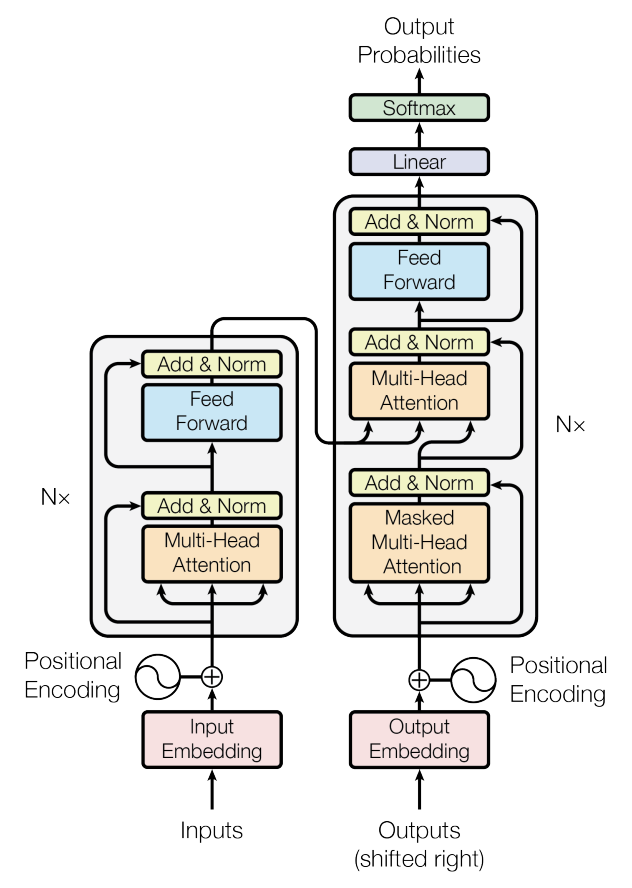
\includegraphics[width=0.4\textwidth]{images/model_architecture/transformer.png}
    \caption{\label{fig:resnet_50_architecture}Transformer Architektur (Quelle: \href{https://arxiv.org/pdf/1706.03762.pdf}{Paper - Attention is all you need})}
\end{figure}


Die Transformer-Architektur \cite{vaswani_attention_2017}, die erstmals im Paper "Attention is All You Need" vorgestellt wurde, ist eine bahnbrechende Methode für das Training von Modellen für Aufgaben der natürlichen Sprachverarbeitung. Sie unterscheidet sich von anderen Modellarchitekturen dadurch, dass sie stark auf das Konzept der "Aufmerksamkeit" (oder genauer, die "Scaled Dot-Product Attention" und "Multi-Head Attention") setzt, anstatt auf die traditionellen rekursiven oder konvolutionellen Schichten.\\\\
Die Kernidee des Transformers ist, dass er gleichzeitig alle Worte oder Tokens in einer Eingabesequenz betrachtet, anstatt sie sequenziell zu durchlaufen. Durch die Berechnung von Aufmerksamkeits-Scores zwischen allen Paaren von Tokens kann das Modell Kontextinformationen aus der gesamten Sequenz erfassen. Dieser Prozess wird in jedem "Transformer Block" durchgeführt, der aus mehreren "Multi-Head Attention"- und "Feed-Forward"-Schichten besteht.\\\\
Diese Architektur ermöglicht es dem Modell, komplexe Muster zwischen den Wörtern in einer Textsequenz zu erfassen, und hat sich als besonders effektiv bei einer Vielzahl von Aufgaben der natürlichen Sprachverarbeitung erwiesen. Sie wurde später auf Bildverarbeitungsaufgaben angewendet, wobei der Vision Transformer ein prominentes Beispiel ist. 


\newpage

\subsection{Modell-Trainingsverfahren}

Um die ausgewählten Modelle erfolgreich für die Klassifizierung der Bilder aus den Kamerafallen einzusetzen, haben wir verschiedenste Pre-processing Schritte der Daten eingeführt, um das Resultat zu optimieren. 

\subsubsection{Data Preprocessing}
Zunächst wird beim Training eine Transformation der Daten vorgenommen. Dies führt dazu, dass sich die Daten und dementsprechend deren Gradient bei jedem Step leicht ändert. Dadurch soll das Modell weniger auf die Trainingsdaten overfitten und gilt somit als eine Regularisierungsstrategie.

\begin{figure}[!h]
    \centering
    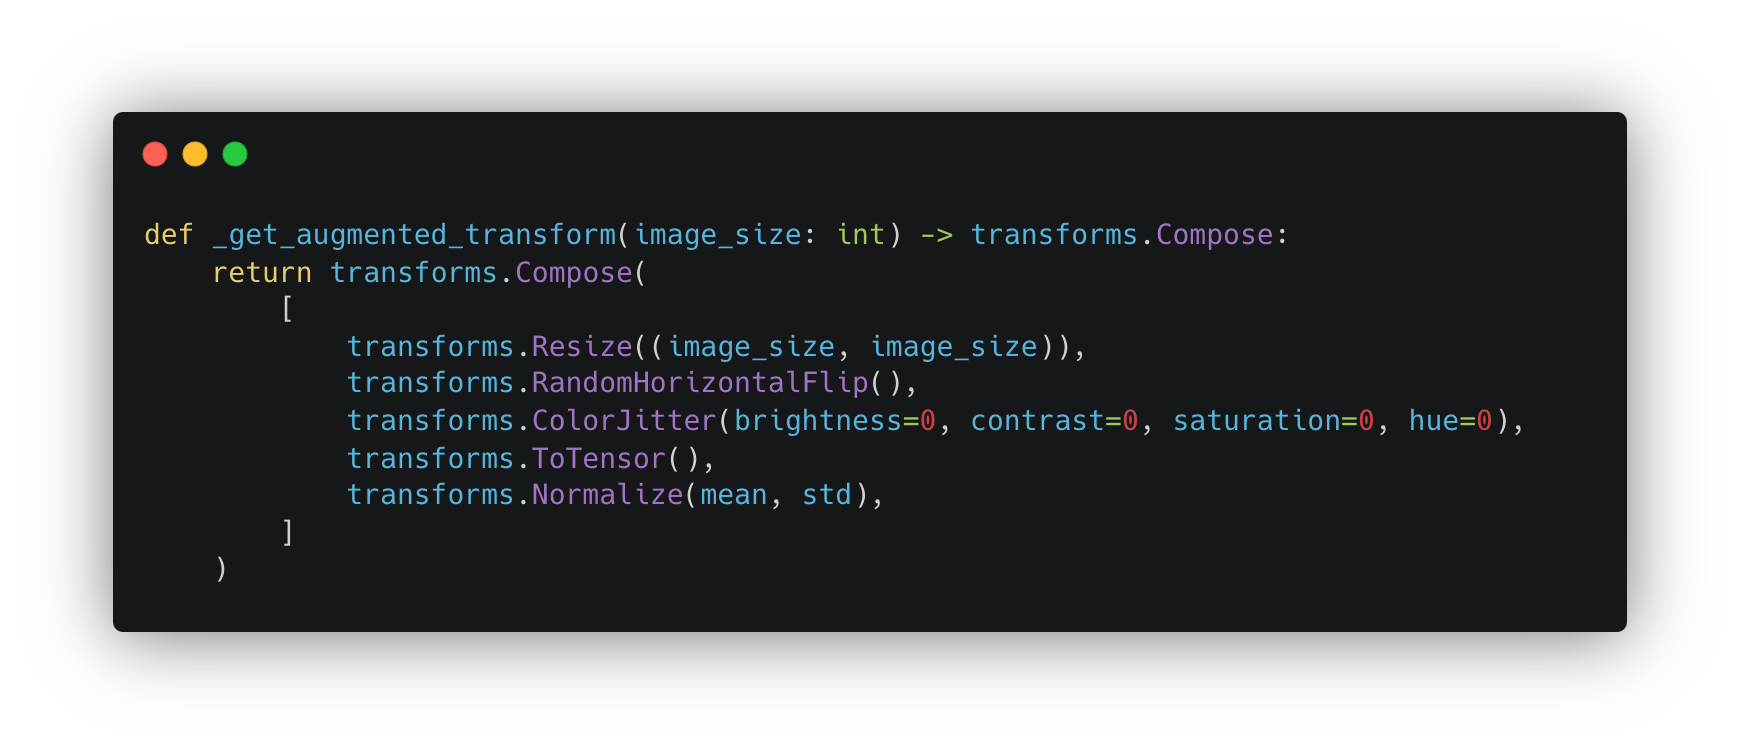
\includegraphics[width=0.6\textwidth]{images/augmented_transformation.png}
    \caption{\label{fig:augmented_transformation}Augmentierte transformation}
\end{figure}

Bei der Transformation der Trainingsdaten wird eine Funktion \texttt{\_get\_augmented\_transform} verwendet, die eine Reihe von Bildverarbeitungsoperationen, sogenannte Transformationen, auf die Bilder anwendet. Die Reihenfolge der Transformationen in der Funktion definiert die Reihenfolge, in der sie auf die Bilder angewendet werden.

\noindent
Die Transformationen umfassen:

\begin{itemize}

\item \textbf{Grössenänderung (Resize)}: Zuerst wird die Grösse jedes Bildes auf die spezifizierte \texttt{image\_size} geändert. Dies stellt sicher, dass alle Bilder die gleiche Grösse haben, was für die meisten Computer Vision-Modelle notwendig ist, da sie feste Eingabeabmessungen benötigen.

\item \textbf{Zufällige horizontale Spiegelung (RandomHorizontalFlip)}: Diese Transformation spiegelt zufällig das Bild horizontal. Dies kann helfen, das Modell robuster gegenüber horizontalen Variationen im Bild zu machen.

\item \textbf{Farbschwankungen (ColorJitter)}: Diese Transformation verändert zufällig die Farbeigenschaften des Bildes. In diesem speziellen Fall werden jedoch keine Veränderungen vorgenommen, da die Parameter für Helligkeit, Kontrast, Sättigung und Farbton alle auf 0 gesetzt sind.

\item \textbf{Umformung zu Tensor (ToTensor)}: Dies konvertiert das Bild (das in der Regel in einem PIL- oder NumPy-Format vorliegt) in einen PyTorch-Tensor, sodass es von PyTorch-Modellen verarbeitet werden kann.

\item \textbf{Normalisierung (Normalize)}: Schliesslich wird das Bild normalisiert, indem der Mittelwert und die Standardabweichung subtrahiert bzw. durch sie geteilt werden. Die Normalisierung hilft, die numerische Stabilität, das Modelltraining zu verbessern und sicherzustellen, dass verschiedene Merkmale auf einer ähnlichen Skala sind. Es ist zu beachten, dass die Werte für mean und std in diesem Codebeispiel nicht gegeben sind, diese würden normalerweise auf spezifische Werte gesetzt, die auf den Datensatz abgestimmt sind, der verwendet wird.

\end{itemize}

\noindent
Diese Transformationen sind Beispiele für Data Augmentation, eine Technik, die verwendet wird, um die Menge und Vielfalt der Trainingsdaten zu erhöhen und so das Modell robuster zu machen und Overfitting zu verhindern.

\newpage

\begin{figure}[!h]
    \centering
    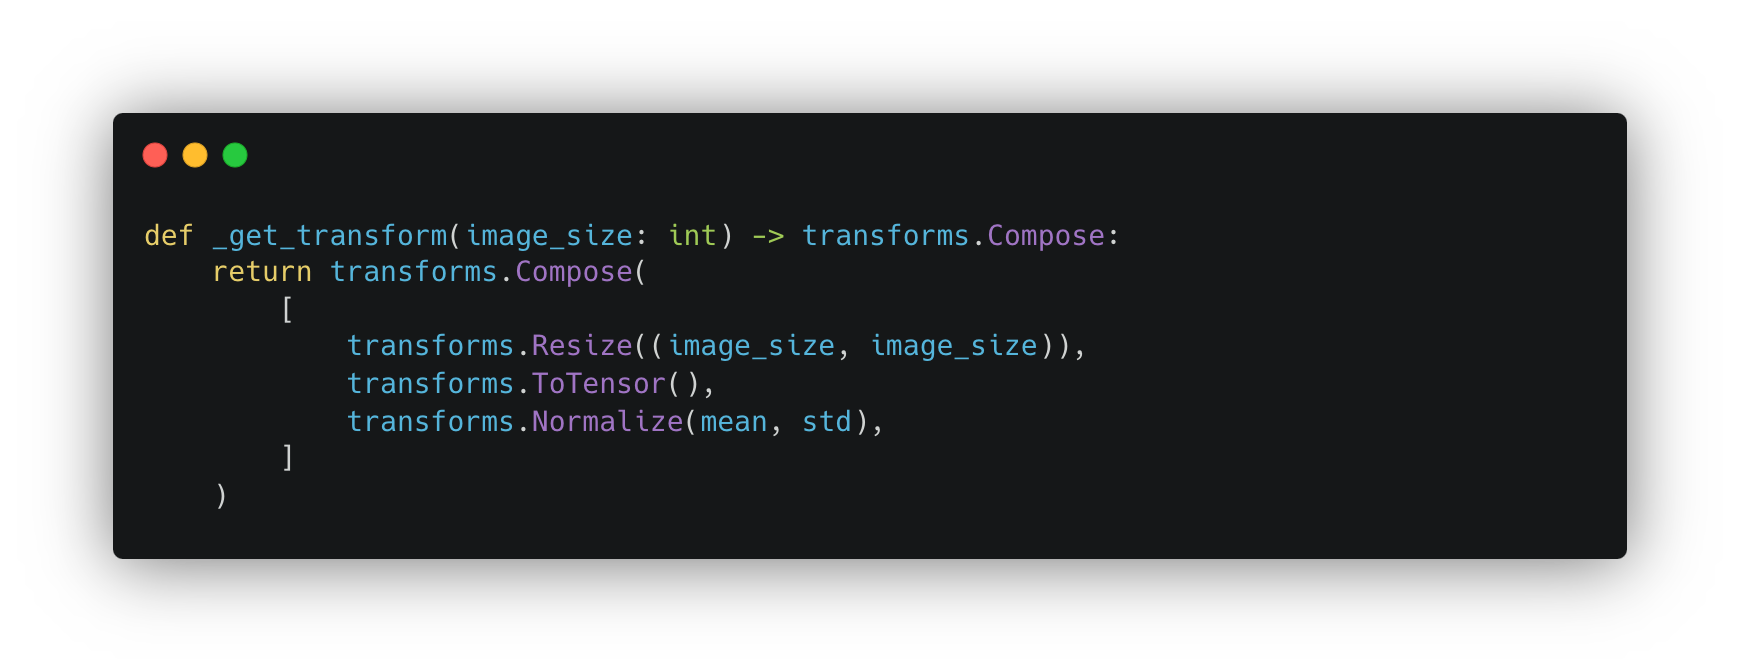
\includegraphics[width=0.6\textwidth]{images/transformation.png}
    \caption{\label{fig:transformation}Transformation von nicht-trainingsdaten}
\end{figure}

Für die Validierungs- und Testdaten verwenden wir eine vereinfachte Variante dieser Transformationen, da wir versuchen diese Daten möglichst genau vorherzusagen und es das Problem von Overfitting in diesem Fall nicht gibt, da das Modell nicht direkt diese Daten lernt. Hier werden nur die \texttt{Resize}, \texttt{ToTensor} und \texttt{Normalize} Transformationen verwendet, um die Validierungs- und Testdaten auf den gleichen Grössen und Farbbereich wie die Trainingsdaten zu bringen.

\subsubsection{Hyperparameter Optimierung}
Zur Optimierung der Hyperparameter haben wir zuerst von Hand pro Modell jeweils einige Parameterkombinationen ausprobiert, um ein Gefühl dafür zu bekommen, welche Parameter bzw. Parameterkombinationen sinnvoll sind. Mit diesem Wissen haben wir dann sogenannte \texttt{Sweeps} auf Weights \& Biases konfiguriert, welche systematisch die verschiedenen Kombinationen der Hyperparameter trainiert und evaluiert. Diese Hyperparameter sind für jedes Modell unterschiedlich.

\begin{figure}[!h]
    \centering
    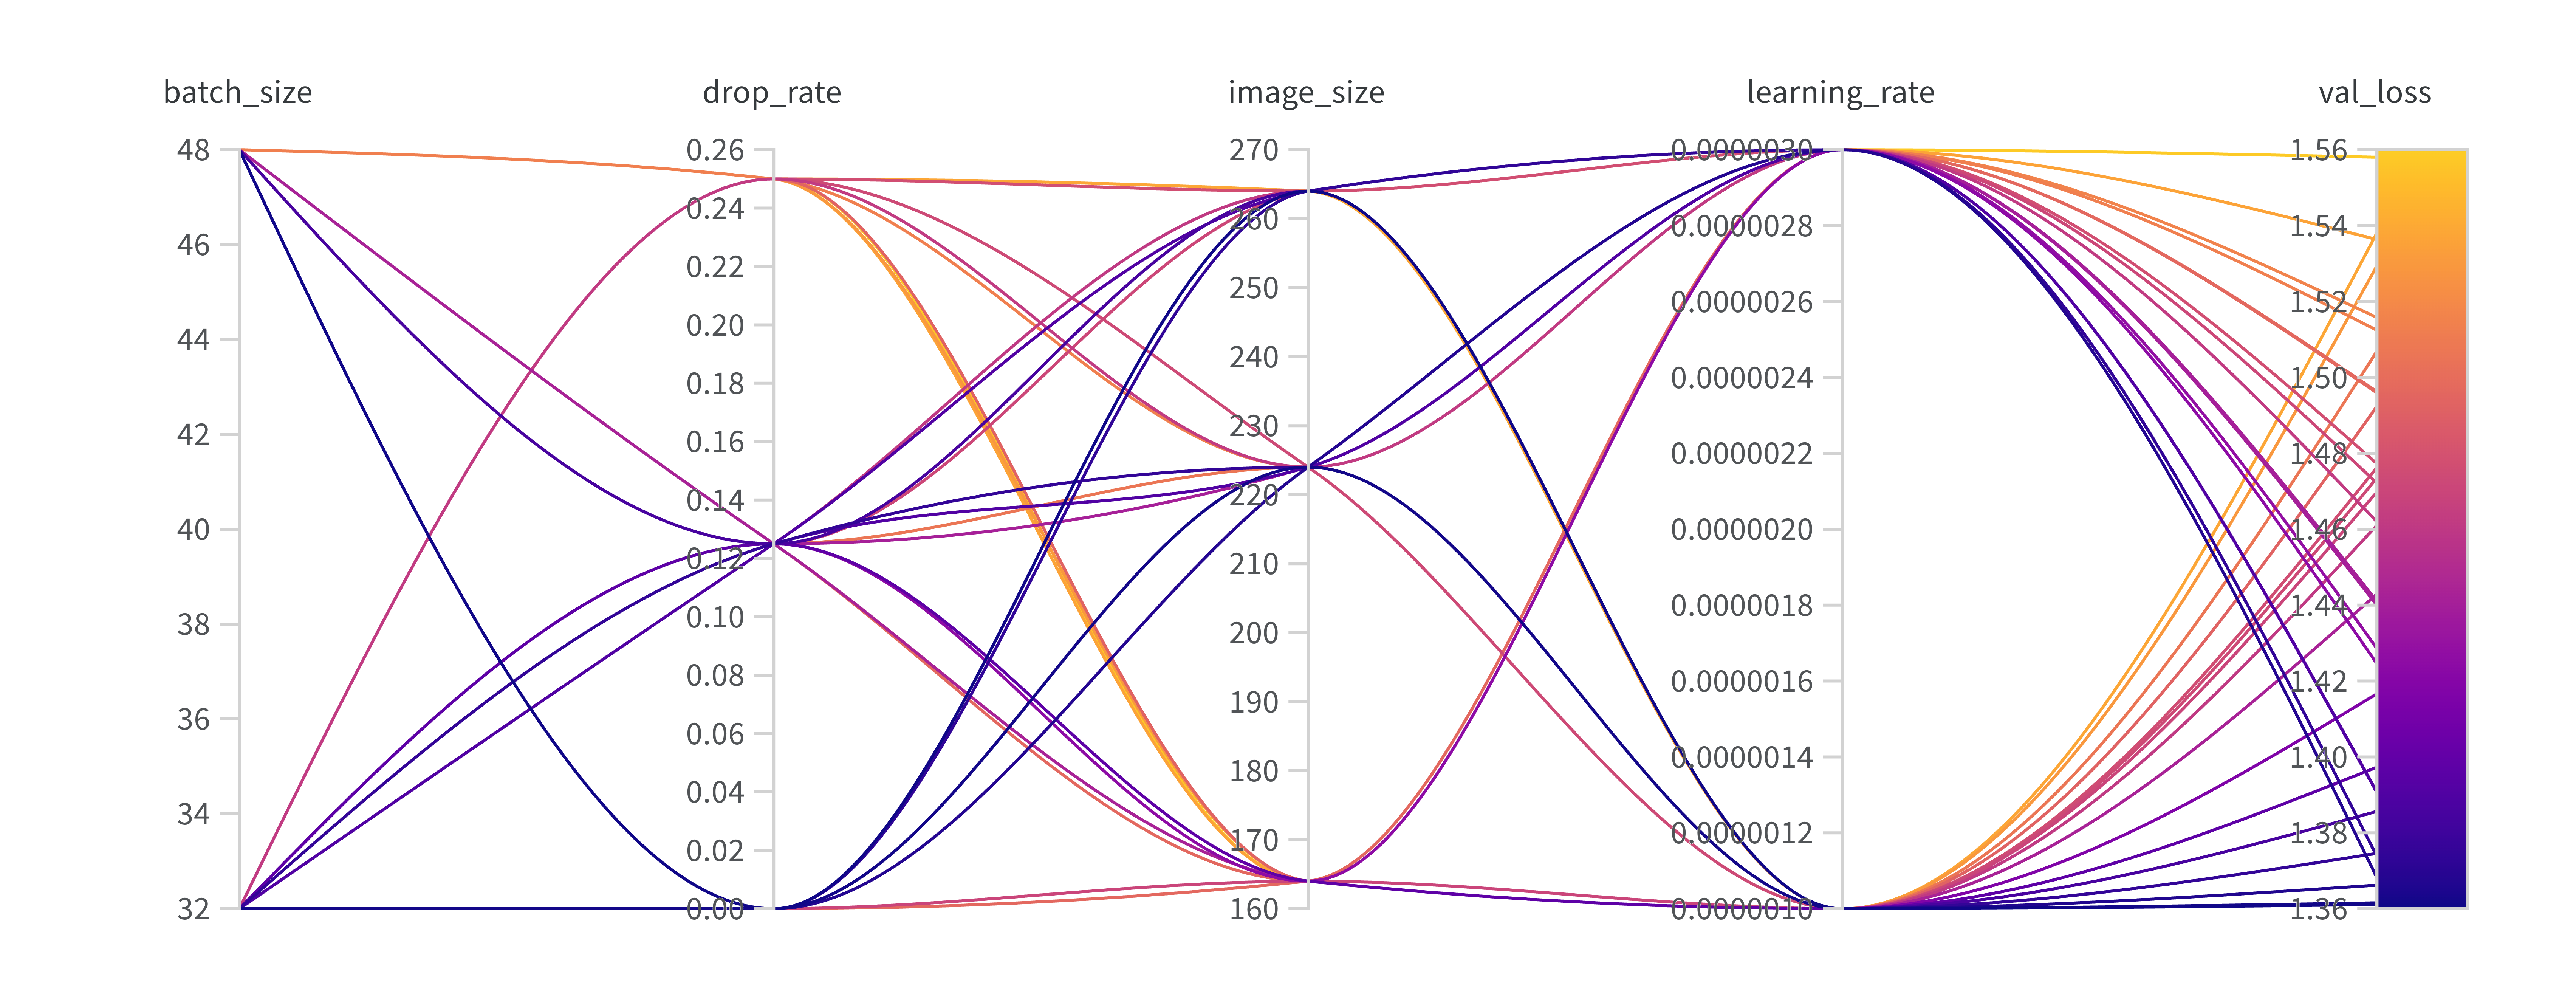
\includegraphics[width=0.8\textwidth]{images/hyperparameter_optimization_example.png}
    \caption{\label{fig:hyperparameter_optimization_example}Beispiel des Resultates einer Hyperparameter Optimierung eines DenseNet161}
\end{figure}

Im Parallel Coordinates Plot in Abbildung \ref{fig:hyperparameter_optimization_example} sieht man, mit welchen Hyperparametern das Modell einen wie guten Validierungsverlust erreicht hat. Wir bei diesem Plot auf Weights \& Biases, mit der Maus über einzelne Runs Hovern und die erreichten Parameter auslesen. Bei diesem Run waren die besten Parameter die folgenden:

\textbf{Batch Size}: 48

\textbf{Drop Rate}: 0.

\textbf{Image Size}: 264

\textbf{Learning Rate}: \mathbf{1e^{-6}}


\noindent
Mit diesen Parametern erreichen wir dann einen Validierungsverlust von \textbf{1.361}. Wenn wir nun genauer auf den Einfluss der verschiedenen Parameter eintauchen möchten, können wir uns den Chart zur Parameter Importance anschauen.

\newpage

\begin{figure}[!h]
    \centering
    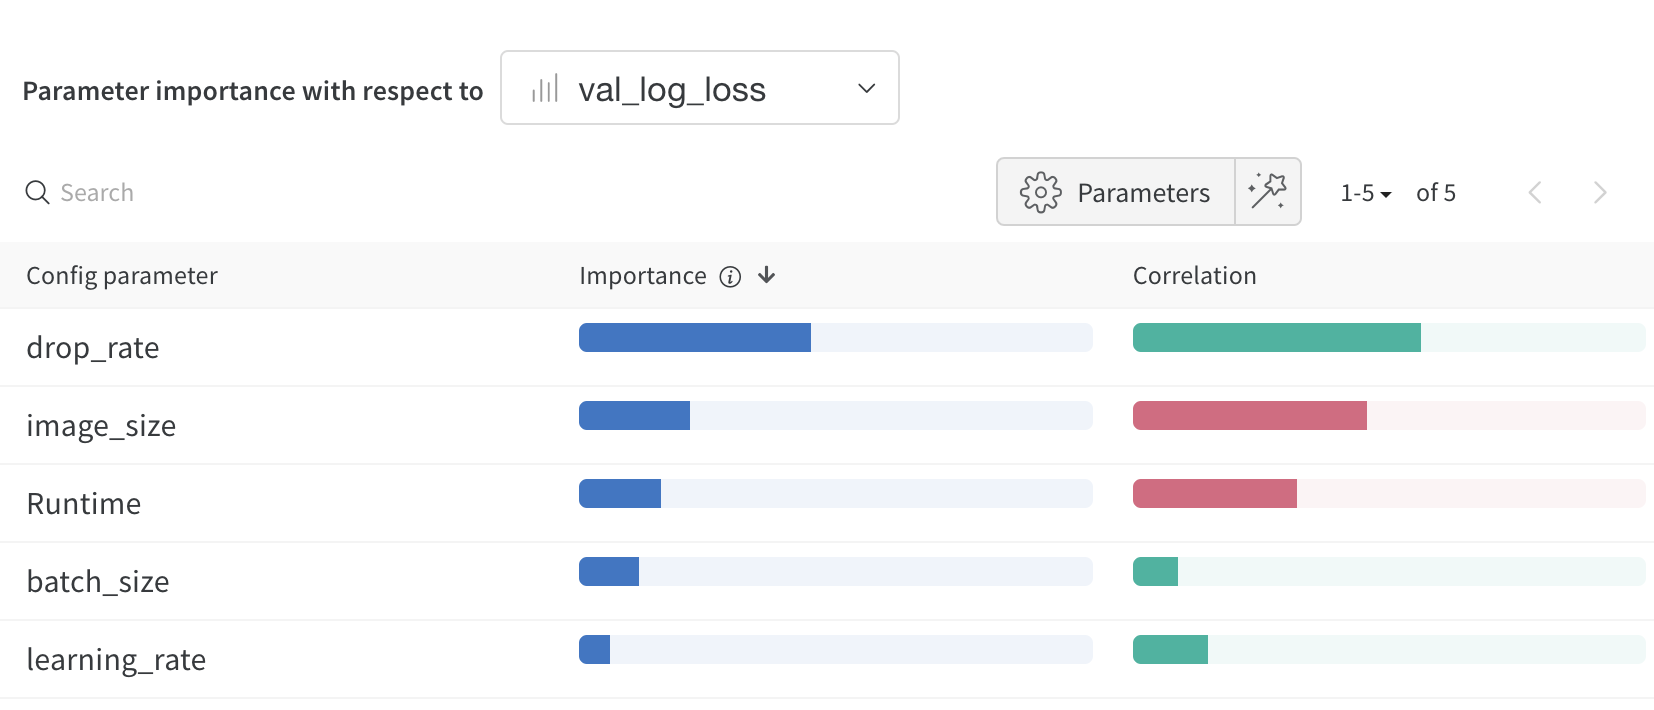
\includegraphics[width=0.8\textwidth]{images/parameter_importance_example.png}
    \caption{\label{fig:hyperparameter_importance_example}Beispiel der Parameter Importance des DenseNet161}
\end{figure}

In Abbildung \ref{fig:hyperparameter_importance_example} sehen wir, welche Parameter einen wie starken Einfluss (berechnet mit Pearson Korrelation) auf das Resultat hat. \\

\textbf{Achtung!} Grün bedeutet hier starke positive Korrelation zwischen dem Parameter und der Zielvariable, da wir versuchen den Validierungs-Verlust zu minimieren, bedeutet der grüne Balken, dass ein höherer Wert dieses Parameters schlechter ist.\\

\noindent
In diesem Beispiel hat beispielsweise \texttt{drop\_rate} und \texttt{image\_size} einen starken Einfluss auf den Validierungs-Verlust.

\subsubsection{Cropping}
Nach ausführlicher Optimierung der Modelle sind wir bei allen Modellen etwa bei einem Validierungsverlust von rund \textbf{1.25} - \textbf{1.30} angestossen. Egal, welche Änderungen wir gemacht haben, haben wir keine Resultate signifikant darunter kamen.
Daher wurde uns bewusst, dass wir drastischere Änderungen an den Modellen und der Vorgehensweise vornehmen müssen, als nur die Hyperparameter zu optimieren.\\\\
\noindent
Ein weitverbreitetes Vorgehen bei der Klassifizierung solcher Subjekte auf den Bildern ist es, ein weiteres Modell, wie Yolo oder Megadetector zu verwenden, um die Bilder auf das Subjekt zuzuschneiden und von diesem zugeschnittenen Bild das Bild zu klassifizieren. Wir haben uns in diesem Fall für Megadetector entschieden, da es bereits auf Kamerafallen vortrainiert ist und wir daraus bessere Resultate erwarten. \\\\
\noindent
Wir haben die Bilder alle einmalig mit dem Megadetector direkt im CameraTraps Repository von Microsoft (\url{https://github.com/microsoft/CameraTraps}) gecropped und danach als Zip File in unserem GitLab Repository abgelegt. Wir sind so vorgegangen, da das Cropping einige Minuten dauert und wir diesen rechenaufwändigen Prozess nicht bei jedem Training wiederholen wollten. Wir haben die Bilder mit certainty thresholds von \textbf{5}, \textbf{10}, \textbf{20}, \textbf{35} und \textbf{50} gecropped.\\\\
\noindent
Diese Dateien haben wir dann per Git LFS in unserem Repository festgehalten und konnten somit einen Hyperparameter für den cropping Threshold bei den Sweeps festlegen.

\newpage

\begin{figure}[!h]
\begin{tabular}{cc}
  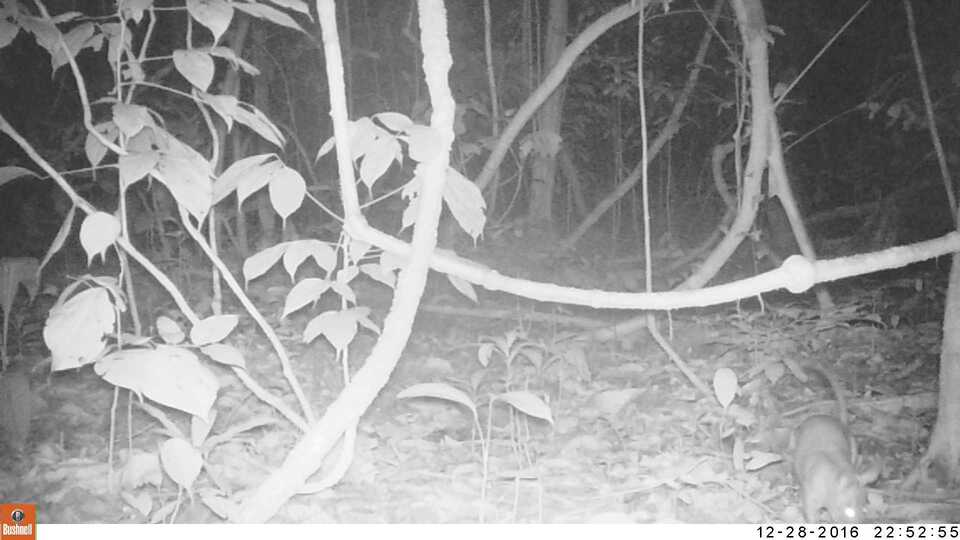
\includegraphics[height=35mm]{images/example_images/ZJ000268.jpg} & 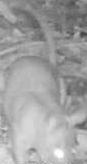
\includegraphics[height=35mm]{images/example_cropped/ZJ000268.jpg} \\
  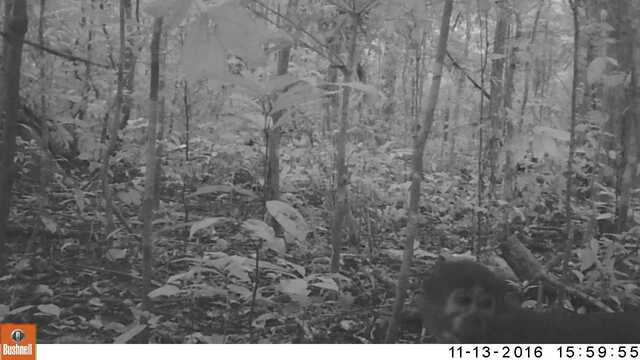
\includegraphics[height=35mm]{images/example_images/ZJ000014.jpg} & 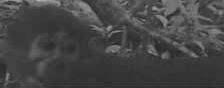
\includegraphics[height=35mm]{images/example_cropped/ZJ000014.jpg}\\
\end{tabular}
\caption{\label{fig:cropped_images_examples}Beispiele von zugeschnittenen Bildern}
\end{figure}

Abbildung \ref{fig:cropped_images_examples} zeigt, dass das cropping mittels Megadetector relativ gute Resultate zeigt. Wir erwarten dadurch eine deutliche Verbesserung des Modelles, da ein Grossteil der irrelevanten Informationen aus dem Datensatz entfernt wird und sich die Modelle auf die relevanten Informationen auf den Bildern fokussieren kann.

\subsection{Ensemble}

Mit dem Ziel, die Stärken unserer Modelle zu vereinen, haben wir ein Ensemble Modell mit 3 Checkpoints der Modelle mit den besten Resultaten erstellt. Dieses Modell predictet einen Dataloader auf den drei Modellen und verwendet die bei Initialisierung festgelegten Gewichte, um den Output der Modelle zu gewichten. Diese Gewichtungen wurden dann ähnlich wie bei der Hyperparameter-Optimierung mit einem Sweep optimiert. 

\newpage

\section{Evaluation}
Die Leistung der Modelle wurde von mehreren Metriken evaluiert: der Accuracy pro Klasse, dem F1-Score (gewichtet, Makro und Mikro) und dem Log-Loss. Durch die Verwendung dieser Metriken können wir ein umfassendes Bild der Modellleistung erhalten. Wir werden in diesem Abschnitt die Leistung unserer Modelle im Detail betrachten.

\subsection{Allgemeine Resultate}

\begin{figure}[!h]
    \centering
    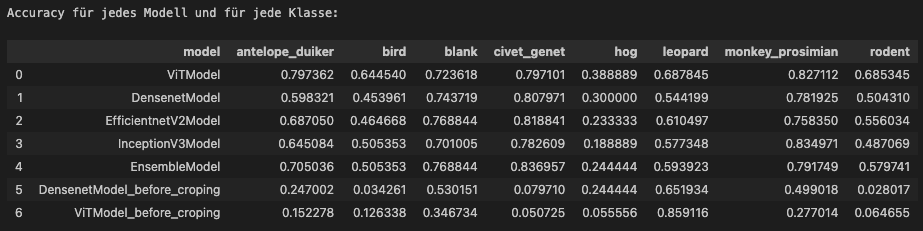
\includegraphics[width=0.9\textwidth]{plots/Accuracy_Tabelle.png}
    \caption{\label{fig:accuracy_table}Accuracy für jedes Modell und Klasse (Tabelle)}
\end{figure}

Die obige Tabelle präsentiert uns die Genauigkeit jedes Modells für jede Klasse. Diese Information kann bedeutungsvoll sein, da sie uns erlaubt, die Stärken und Schwächen der einzelnen Modelle genau zu analysieren. Im Hinblick auf zukünftige Schritte können wir diese Erkenntnisse nutzen und sie in die Entwicklung neuer Modelle einfliessen lassen.

\begin{figure}[!h]
    \centering
    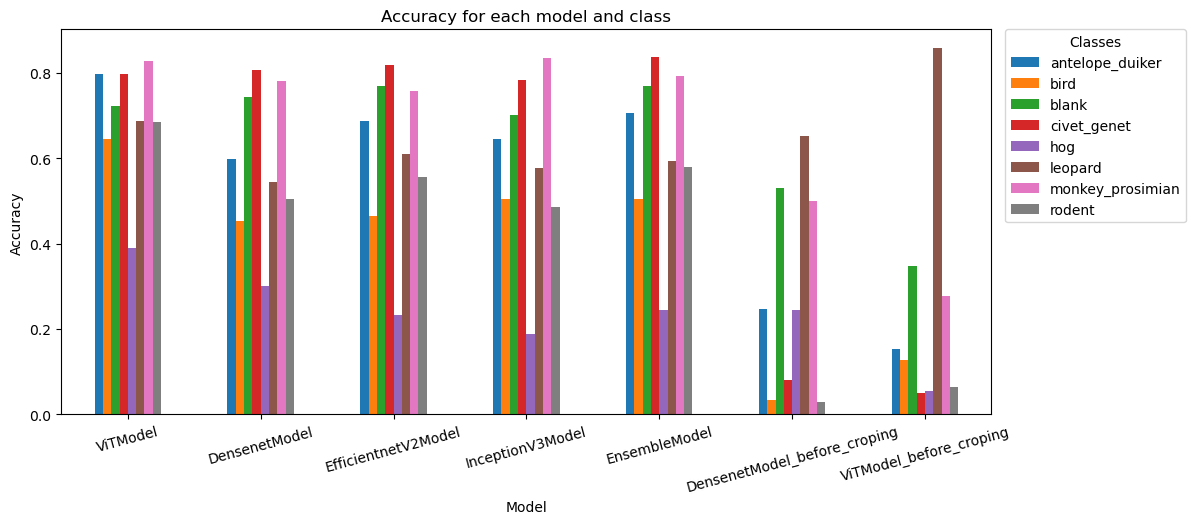
\includegraphics[width=0.9\textwidth]{plots/Accuracy_Barplot.png}
    \caption{\label{fig:accuracy_barplot}Accuracy für jedes Modell und Klasse (Säulendiagramm)}
\end{figure}

In diesem Säulendiagramm sehen wir eine visuelle Darstellung der zuvor dargestellten Tabelle. Es bietet uns eine anschauliche und leicht verständliche Übersicht der Genauigkeit jedes Modells pro Klasse. Die Säulenhöhe repräsentiert hierbei die jeweilige Genauigkeit, und jede Farbe repräsentiert eine andere Klasse. Auf diese Weise können wir auf einen Blick die Stärken und Schwächen der verschiedenen Modelle in Bezug auf die unterschiedlichen Klassen erfassen und Vergleiche anstellen. Wir sehen bereits hier, dass das ViT Modell einen deutlich besseren Score, als die anderen Modelle erreicht.

\newpage

\begin{figure}[!h]
    \centering
    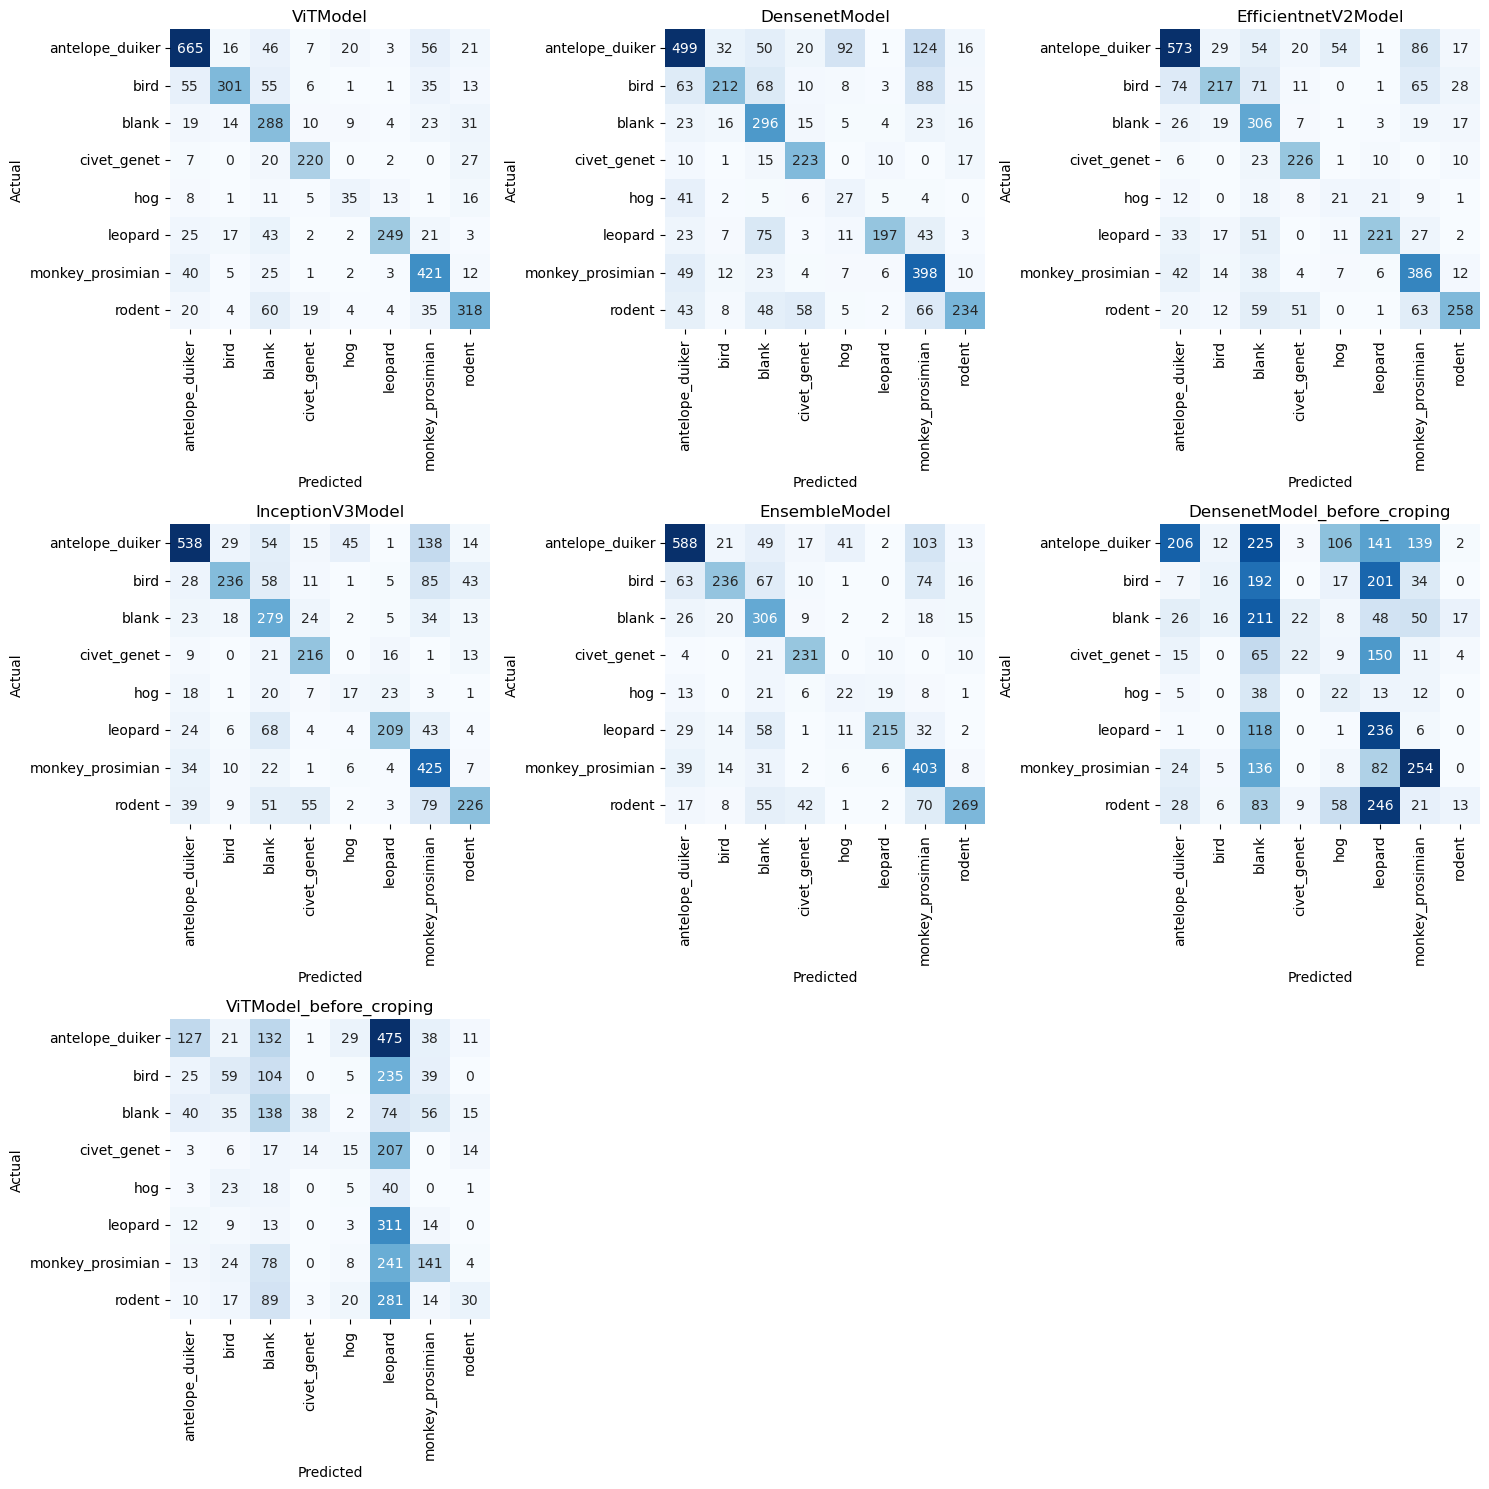
\includegraphics[width=1\textwidth]{plots/Confusionmatrix.png}
    \caption{\label{fig:confusion_matrix}Confusion-Matrizen für alle Modelle}
\end{figure}

Abbildung \ref{fig:confusion_matrix} zeigt für jedes Modell eine Confusion Matrix. Die Confusion Matrix ist ein leistungsstarkes Werkzeug, das uns eine detaillierte Darstellung der Leistung jedes Modells bietet. Auf der Hauptdiagonalen können wir die korrekten Vorhersagen des Modells ablesen, während die restlichen Elemente die Fehlklassifikationen darstellen.\\\\
Durch diese Darstellung lässt sich ausgezeichnet erkennen, welche Klassen das Modell zuverlässig identifizieren kann und wo es Schwierigkeiten hat. Hierdurch gewinnen wir wertvolle Einsichten in die spezifischen Bereiche, in denen Verbesserungen notwendig sind, und könnten so in Zukunft gezielte Optimierungsmassnahmen durchführen. Es ermöglicht uns ausserdem, die Beziehung zwischen verschiedenen Klassen zu verstehen und mögliche Verwechslungen zu identifizieren, die bei der Klassifikation auftreten können.\\\\
In den bisherigen Grafiken wurden die Genauigkeiten (Stärken und Schwächen) der einzelnen Modelle dargestellt, die Resultate werden in den nächsten Abschnitten genauer untersucht.

\subsection{Die besten Modelle vor dem Cropping}

\subsubsection{DenseNet}

\begin{figure}[!h]
    \centering
    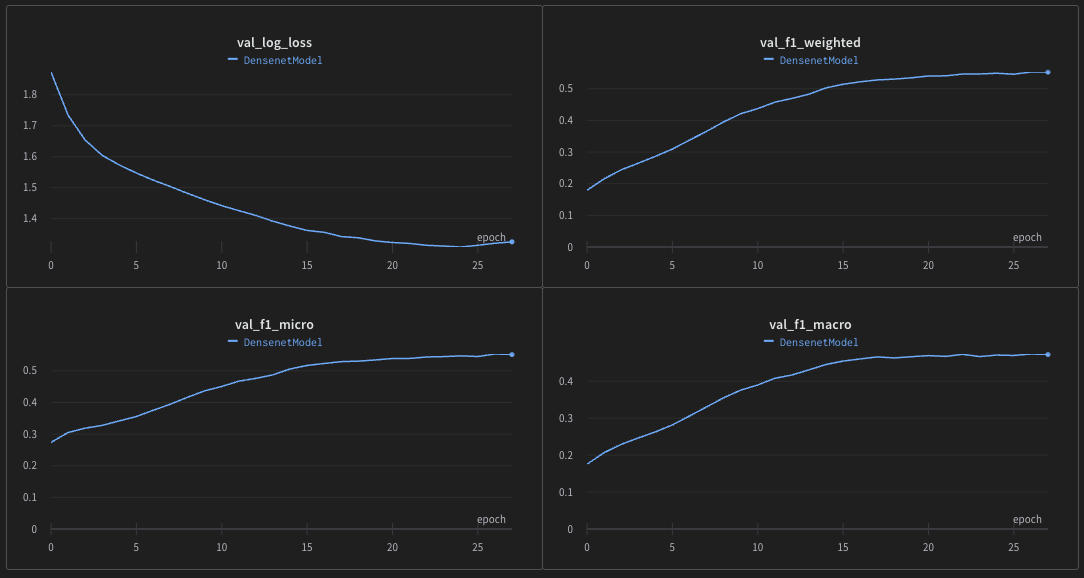
\includegraphics[width=0.8\textwidth]{plots/DenseNet_wandb_before_cropping.png}
    \caption{\label{fig:wb_densenet_before_cropping}Verlauf der DenseNet Metriken (vor dem Cropping)}
\end{figure}

Dieser Report aus Weights \& Biases zeigt das beste Modell für die Bilder vor ihrer Zuschneidung (Cropping). Es ist deutlich zu erkennen, dass selbst unser bestes Modell ein Log Loss von lediglich 1.309 erreicht.\\\\
Im Vergleich zu den anderen Modellen in Abbildung \ref{fig:confusion_matrix} wird schnell klar, dass die Genauigkeit pro Klasse bei den Bildern vor dem Cropping deutlich niedriger ist. Zudem unterscheidet sich die Verteilung der am besten vorhergesagten Klasse merklich. Innerhalb dieses Modells erweisen sich die Kategorien 'blank' und 'leopard' als genauste, während 'bird' als schwächste Klasse erscheint.

\subsubsection{ViTModel}

\begin{figure}[!h]
    \centering
    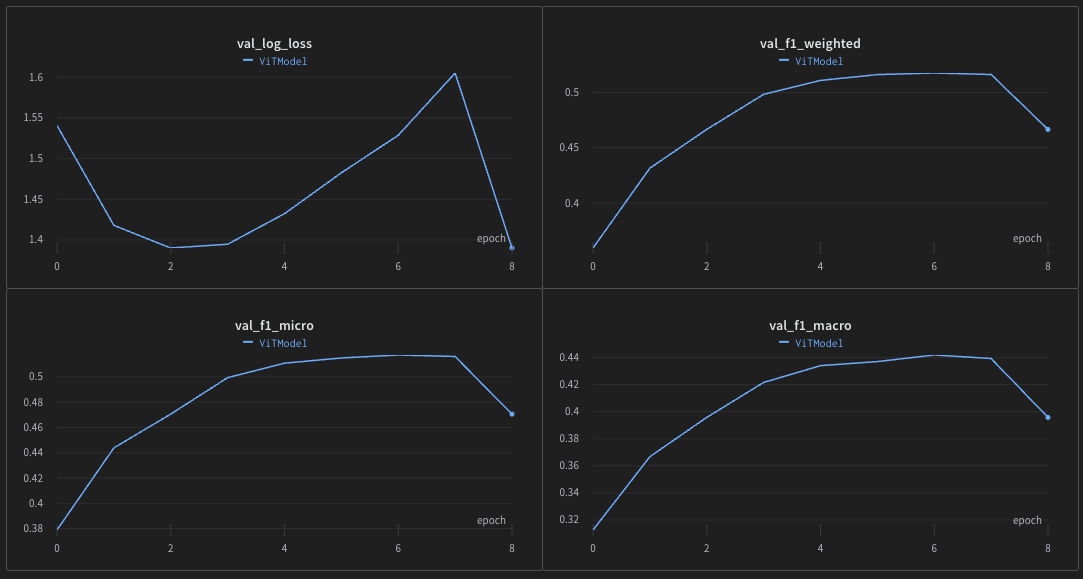
\includegraphics[width=0.8\textwidth]{plots/ViT_Model_wandb_before_cropping.png}
    \caption{\label{fig:wb_vitmodel_before_cropping}Verlauf der ViT-Models Metriken (Vor dem Cropping)}
\end{figure}

Unser ViTModel, das insgesamt unser bestes Modell darstellt, schneidet mit einem val\_log\_loss von 1.39 überraschenderweise auf den ursprünglichen Bildern deutlich schlechter ab als das DenseNet. Die Erkennung der einzelnen Klassen fällt hier ebenfalls weniger präzise aus als bei den anderen Modellen, die nach dem Croppen trainiert wurden. \\\\
Hier hätte einen ausführliche Hyperparameteroptimierung mit hoher wahrscheinlchkei noch zu besseren Resultaten füren können, welche das DenseNet wahrscheinlich auch überholt minimal hätten. An diesem Punkt wurde jedoch klar, dass drastischere Mittel notwendig sind, um eine deutlich bessere Leistung zu erreichen. Desshalb haben wir uns auf das Cropping fokussiert.\\\\
Dennoch bietet es eine bemerkenswerte Überraschung: Die Klasse 'leopard' wird mit einer Genauigkeit von 85\% erstaunlich gut identifiziert. Dies stellt die beste Vorhersage aller Modelle dar. Im Gegensatz dazu sind 'civet\_genet' und 'hog' die am schlechtesten performenden Klassen, mit einer Genauigkeit von lediglich 5\% genauer gesagt 5,5\%.

\subsection{Modelle nach dem Cropping}

\subsubsection{ViTModel}

\begin{figure}[!h]
    \centering
    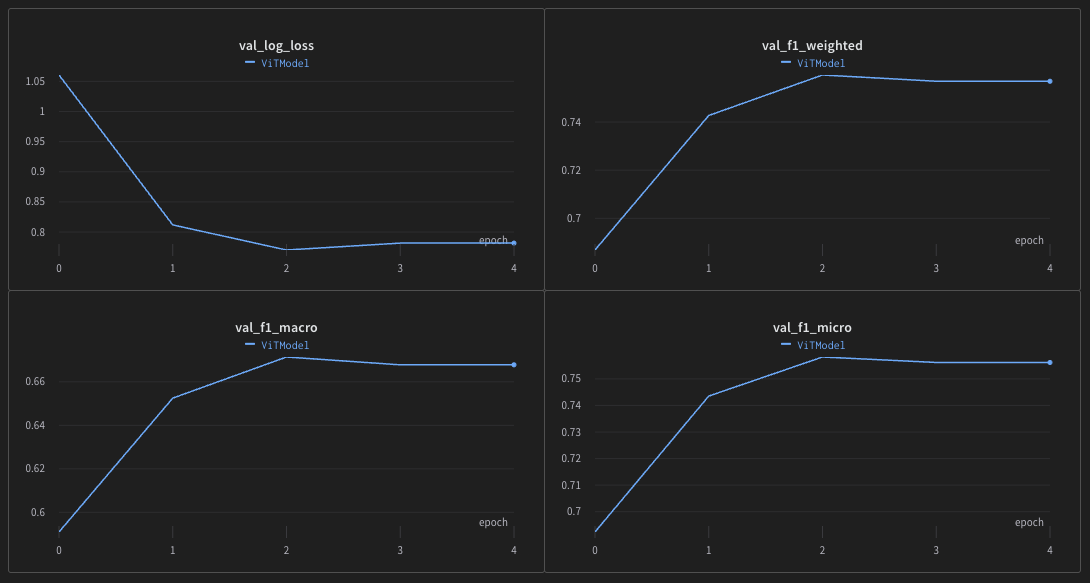
\includegraphics[width=0.8\textwidth]{plots/ViT_Model_wandb.png}
    \caption{\label{fig:wb_vitmodel}Verlauf der ViT-Models Metriken}
\end{figure}

Das ViTModel hat sich nach dem Cropping im Vergleich zu den anderen Modellen als das Überlegen erwiesen. Mit einem F1-Weighted von 0,7569, einem F1-Makro von 0,6678 und einem F1-Mikro von 0,7562 zeigt das ViTModel, dass es eine solide Leistung über alle Klassen hinweg bietet. Der Log-Loss von 0,7816 deutet ebenfalls darauf hin, dass das ViTModel über eine gute Klassifizierungsleistung verfügt.\\\\
Ausserdem kann man aus Abbildung \ref{fig:accuracy_table} entnehmen, dass das ViTModel bei der Klassifizierung von 'antelope\_duiker', 'civet\_genet' und 'monkey\_prosimian' jeweils eine Accuracy von mindestens 80\% erreicht hat, was hervorragende Ergebnisse auf unserem Datensatz sind. Die schlechteste Accuracy wurde bei der Klasse 'hog' erreicht, da dies aber bei fast allen Modellen der Fall war, spricht dies dafür, dass 'hog' eine schwierig zu klassifizierende Klasse sein muss. Ein Grund dafür könnte sein, dass die Klasse 'hog' mit Abstand am wenigsten im Datensatz vertreten ist.

\newpage

\subsubsection{DenseNet}

\begin{figure}[!h]
    \centering
    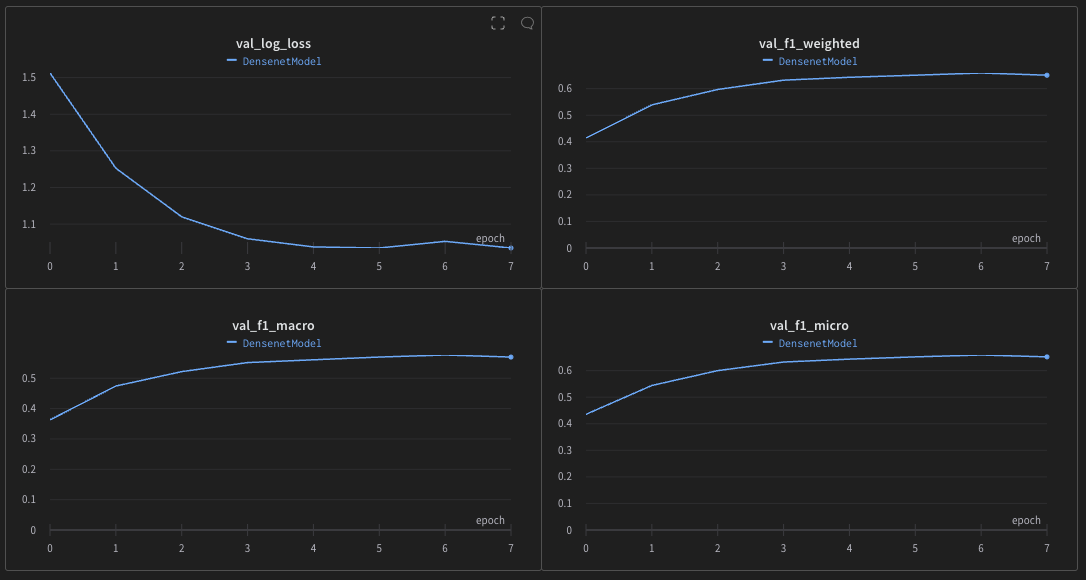
\includegraphics[width=0.7\textwidth]{plots/DenseNet_wandb.png}
    \caption{\label{fig:wb_densenet}Verlauf der DenseNet Metriken}
\end{figure}

Im Vergleich zum ViTModel hat das DensenetModel in allen Metriken eine geringere Leistung gezeigt. Der F1-Weighted-Score lag bei 0,6507, der F1-Makro bei 0,5698 und der F1-Mikro bei 0,6518. Der Log-Loss war mit 1,035 vergleichsweise höher, was auf eine geringere Klassifizierungsgenauigkeit hinweist. Trotzdem hat das DensenetModel bei der Klassifizierung der Klasse 'Monkey\_Prosimian' mit einer Genauigkeit von 0,815324 immer noch gut abgeschnitten.

\subsubsection{EfficientNet}

\begin{figure}[!h]
    \centering
    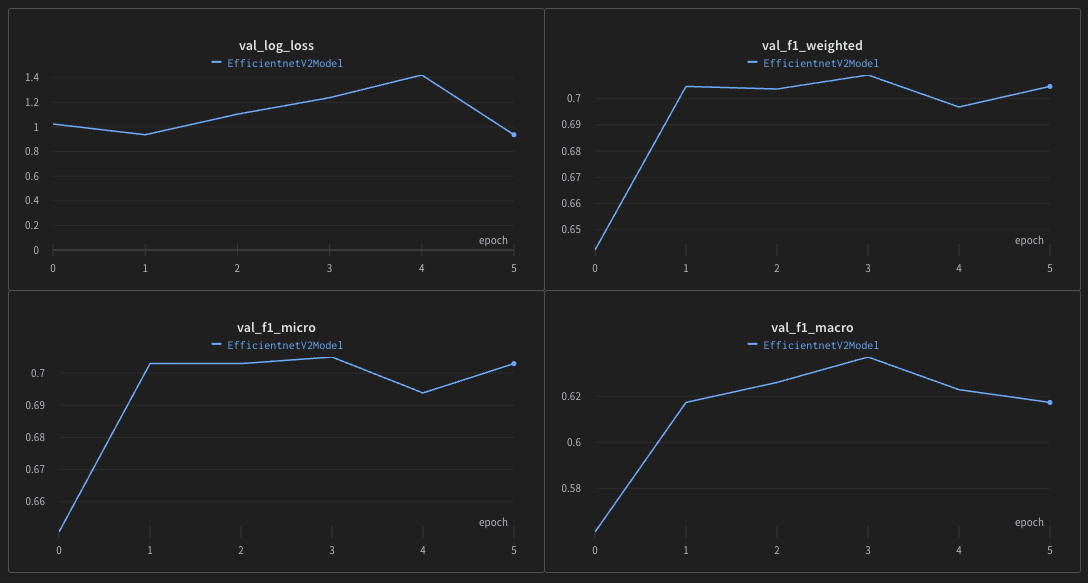
\includegraphics[width=0.7\textwidth]{plots/EfficientNet_wandb.png}
    \caption{\label{fig:wb_efficient}Verlauf der EfficientNet Metriken}
\end{figure}

Das EfficientnetV2Model hat ebenfalls gute Ergebnisse erzielt, allerdings mit etwas niedrigeren Genauigkeitswerten als das ViT. Der F1-Weighted-Score lag bei 0,7047, der F1-Makro bei 0,6173 und der F1-Mikro bei 0,7029. Der Log-Loss von 0,9368 war ebenfalls etwas höher als der des ViTModells. Dennoch hat es von allen nicht-Transformer-Modellen die beste Leistung gezeigt.\\\\
Ebenfalls ist es spannend zu sehen, dass das EfficientNet mit dem Ensemble-Modell die einzigen beide Modelle sind, die als Best-Vorhergesagte-Klasse nicht 'monkey\_prosimian' haben, sondern 'civet\_genet'. Somit kann man schlussfolgern, dass das EfficientNet und das Ensemble-Modell die Klasse 'civet\_genet' besser klassifizieren können als die anderen Modelle. Diese Erkenntnis könnte für weitere Ensemble-Methoden unter Umständen hilfreich sein.


\subsubsection{Inception}

\begin{figure}[!h]
    \centering
    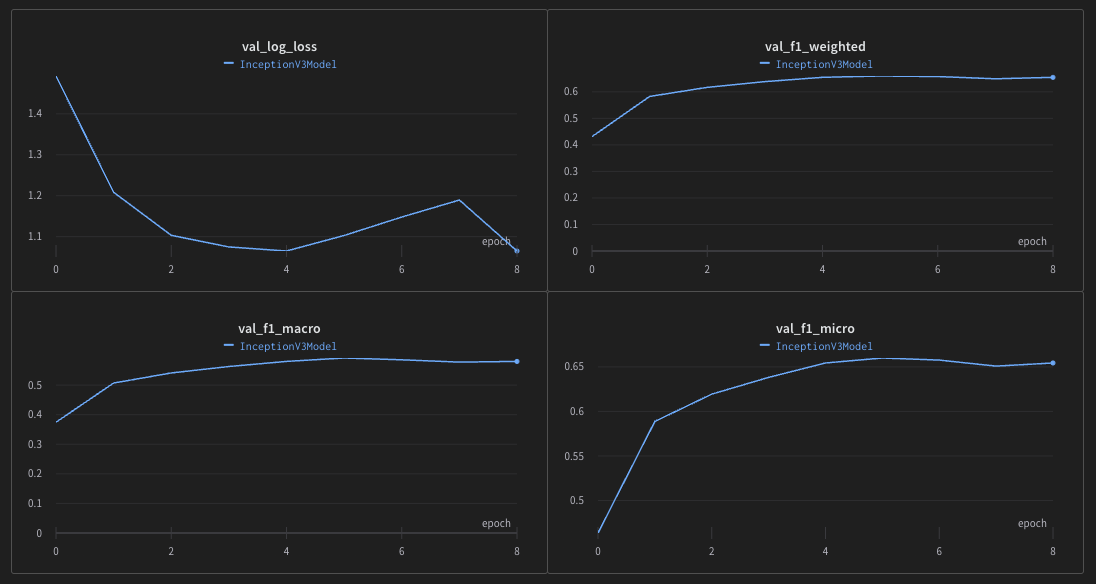
\includegraphics[width=0.8\textwidth]{plots/Inception_wandb.png}
    \caption{\label{fig:wb_inception}Verlauf der Inception Metriken}
\end{figure}

Die Leistung des InceptionV3Model war im Vergleich zu den anderen Modellen nicht besonders gut.\\\\
Der F1-Weighted-Score betrug 0,6546, der F1-Makro bei 0,5801 und der F1-Mikro bei 0,6544. Der Log-Loss von 1,065 konnte ebenfalls nicht überzeugen. Bei den Genauigkeiten pro Klasse in Abbildung \ref{fig:accuracy_table} verhält sich das Inception-Modell ähnlich wie das DenseNet-Modell, mit Ausnahme, dass es 'monkey\_prosimian' deutlich besser klassifizieren konnte, jedoch 'hog' deutlich schlechter.

\subsubsection{Ensemble}

\begin{figure}[!h]
    \centering
    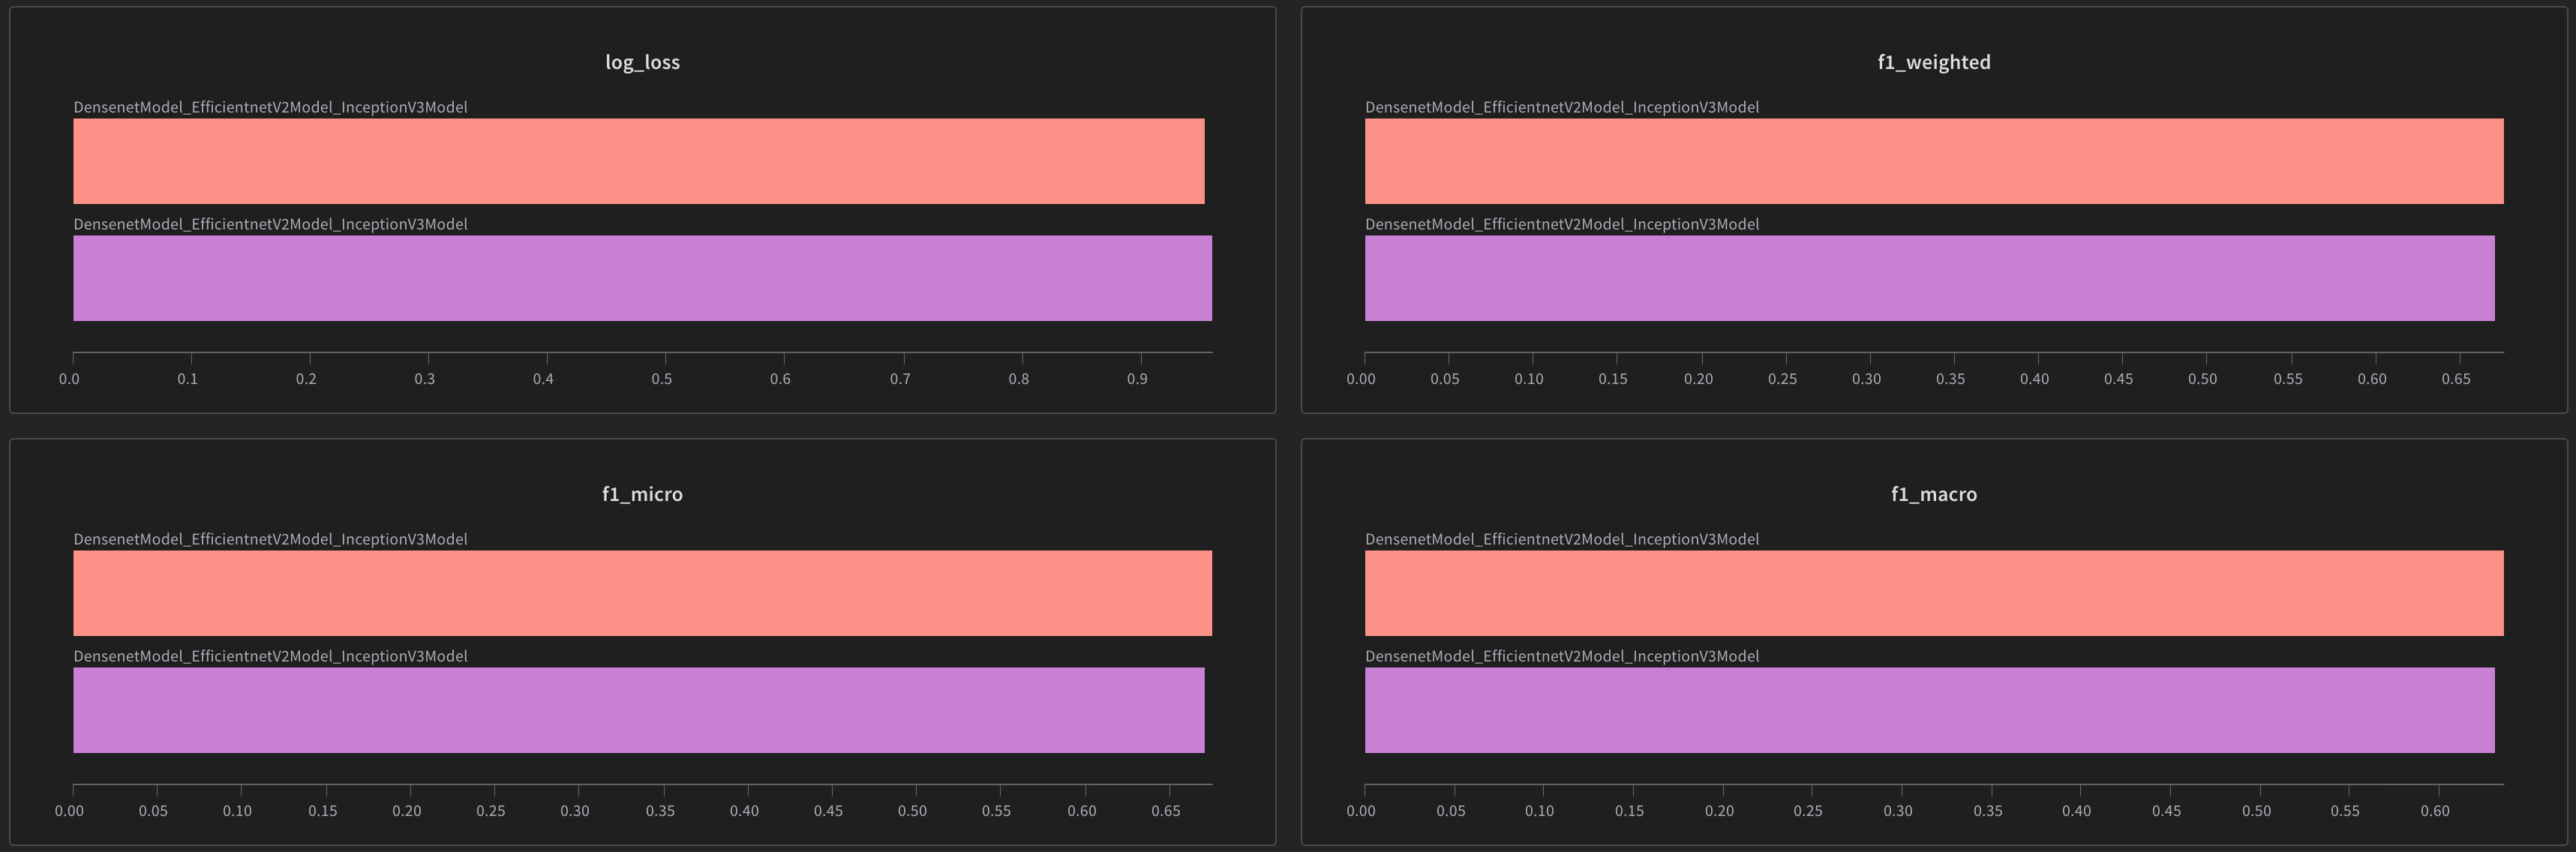
\includegraphics[width=1.0\textwidth]{plots/Ensemble.png}
    \caption{\label{fig:wb_ensemble}Verlauf der Ensemble-Metriken}
\end{figure}

In Abbildung \ref{fig:wb_ensemble} sind die Resultate aus dem besten (oben) und schlechtesten (unten) unserer Ensemble-Modelle zu sehen. Sie basieren alle aus einer gewichteten Kombination des DensetNet, EfficientNet und InceptionV3 Modelle. Diese Ensemble-Modelle konnten in vielen Metriken mit dem EfficientNet mithalten, z. B. konnte es mit dem F1-Makro (0,6416) und dem F1-Mikro (0.6794) das EfficientNet schlagen, jedoch sind Log-Loss (0,9489) und F1-Weighted (0,6808) trotzdem höher als die des EfficientNets. Die Accuracy pro Klasse ist ebenfalls ähnlich wie beim EfficientNet, jedoch konnte das Ensemble-Modell 'rodent' besser klassifizieren als das EfficientNet.\\\\
Auch in Abbildung \ref{fig:accuracy_barplot} ist zu sehen, dass das Ensemble Modell keine signifikanten Verbesserungen im Gegensatz zu unseren anderen Modellen erreichte.

\subsection{Fazit}
Nach eingehender Analyse dieser Modelle und dem Vergleich untereinander, lässt sich eindeutig feststellen, dass das Zuschneiden der Bilder einen signifikanten Einfluss auf die Modellleistung hat. Die verbesserte Performance nach dem Croppen bestätigt die Wichtigkeit dieses Prozesses bei der Vorverarbeitung der Bilddaten, um irrelevante Bildinformationen zu eliminieren und den Fokus auf die relevantesten Merkmale zu lenken. Dies unterstreicht die Notwendigkeit, kontinuierlich die Datenaufbereitungsstrategien zu optimieren und anzupassen, um die bestmöglichen Ergebnisse zu erzielen.

\subsection{Schlussfolgerung}
Alle Modelle zeigen eine beeindruckende Leistung bei der Identifizierung bestimmter Klassen, wobei bei anderen Klassen eine Verbesserung wünschenswert ist. Ein übergreifendes Problem ist die Klassifizierung der Kategorie 'hog', die bei allen Modellen eine niedrige Genauigkeit aufweist.\\\\
Die Klassifizierung der Klasse 'hog' könnte durch eine weitere, tiefere Untersuchung der Daten evtl. noch verbessert werden. Da diese Klasse mit Abstand am wenigsten im Datensatz vertreten ist, könnte man versuchen, mehr Daten für diese Klasse zu sammeln oder weitere Datenvermehrungstechniken verwenden, sowie das Kopieren der Daten, die dann leicht geändert werden, um Overfitting zu vermeiden.\\\\
Wir sind insgesamt sehr zufrieden mit den Ergebnissen unserer Modelle. Alle Modelle haben eine angemessene Leistung erbracht, insbesondere bei der Klassifizierung der 'monkey\_prosimian'-Klasse. Das ViT-Modell sticht dabei besonders hervor, sowohl hinsichtlich der Genauigkeit als auch der F1-Scores und des Log-Loss. Diese Leistung zeigt die Effektivität der Transformer-Architektur Modells auch im Bereich der Bildklassifizierung und bestätigt seine Stärken in der Verarbeitung von Bildinformationen und zeigt, wie mächtig die Transformer-Architektur für bildklassifizierung sein kann.\\\\
Trotz einiger Verbesserungsmöglichkeiten, wie das vertiefte Untersuchen der 'hog' Klasse oder weiteren Ensemble-Methoden (einzelne Modelle für einzelne Klassen) sowie zusätzlicher Transformer-Modelle auszutesten, unterstreichen diese Ergebnisse den Erfolg unserer Arbeit und die Qualität unserer Modelle.

\subsubsection{Leaderbord von drivendata}
Mit unserer Teilnahme an der Competition "Conser-vision Practice Area: Image Classification" und den Resultaten können wir bestätigen, dass Deep Learning die Klassifikation von Aufnahmen von Wildtierkameras unterstützen kann.

\begin{figure}[!h]
    \centering
    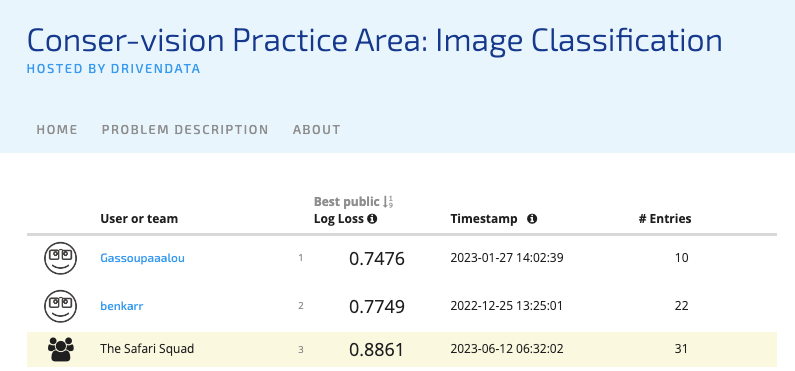
\includegraphics[width=0.6\textwidth]{plots/Leaderboard_Competition.png}
    \caption{\label{fig:leaderboard_competition}Screenshot des Leaderboards, Stand: 17.06.2023, 17:08. (Website: \href{https://www.drivendata.org/competitions/87/competition-image-classification-wildlife-conservation/leaderboard/?page=1}{drivendata.org})}
\end{figure}
Abschliessend möchten wir erwähnen, dass wir uns über den dritten Platz in dieser globalen Competition enorm freuen. Es ist uns gelungen, uns gegen eine starke Konkurrenz durchzusetzen und uns unter den Top 3 zu platzieren. Dieses Ergebnis würdigt die Qualität unserer Arbeit und motiviert uns, weiterhin nach Exzellenz zu streben.

\newpage

\bibliographystyle{plain}
\bibliography{ccv1}

\end{document}
